\chapter{Differentialrechnung in $\R^{\lowercase{n}}$}
\section{Partielle Ableitungen und Differential}
Wie kann man die Begriffe der \todo{Missing content?? page 113 top} Differentialrechnung auf Funktionen $f:\Omega \subset \R^n\to\R$ erweitern?\\

Funktionen in mehreren Variablen sind ein \emph{bisschen} komplizierter als Funktionen in einer Variable.
\subsubsection*{Beispiel}
\begin{enumerate}
\item $f(x)=x^2+5$ ist im Ursprung stetig, da $\lim\limits_{x\to 0}f(x)=f(0)$. Aber $f:\R^2\to\R$ \[f(x,y) = \left\{ {\begin{array}{*{20}{c}}
{\frac{xy}{{x^2} + {y^2}}}&{(x,y)\not  = (0,0)}\\
0&{(x,y) = (0,0)}
\end{array}} \right.\] ist im Ursprung nicht stetig. %page 114 top
\todo{Where is number 2 of the beispiel??}
\end{enumerate}
\todo{is this continuation of the Beispiel, or is it outside??}
\begin{figure}[ht]
\begin{minipage}[b]{0.45\linewidth}
\centering
\[\lim_{\substack{x \to 0 \\ y = 0}}{\frac{x \cdot y}{x^2 + y^2}} = 0 = f(0,0)\]
\end{minipage}
\hspace{0.5cm}
\begin{minipage}[b]{0.45\linewidth}
\centering
\[\lim_{\substack{y \to 0 \\ x = 0}}{\frac{x \cdot y}{x^2 + y^2} = 0 = f(0,0)}\]
\end{minipage}
\end{figure}

Aber der Limes entlang der Gerade $y=mx$
\[\mathop {\lim }\limits_{\begin{array}{*{20}{c}}
{x \to 0}\\
{y \to 0}\\
{y = mx}
\end{array}} f(x,mx) = \mathop {\lim }\limits_{x \to 0} \frac{{m{x^2}}}{{(1 + {m^2}){x^2}}} = \mathop {\frac{m}{{1 + {m^2}}}}\limits_{\begin{array}{*{20}{c}}
 \downarrow \\
{{\text{Hängt von }} m {\text{ ab}}}
\end{array}} \]
und $\frac{m}{1+m^2}\not=0$, falls $m\not=0$. Eine Funktion $f(x,y)$ an der Stelle $(x_0,y_0)$ ist stetig wenn der Limes $\mathop {\lim }\limits_{(x,y) \to ({x_0},{y_0})} f(x,y)$ in jeder Richtung den gleichen Wert hat.
\begin{definition}{8.1}
Sei $\Omega\subset\R^n$, $f:\Omega \to\R$, $a\in\Omega$
\begin{enumerate}
\item $f$ hat den Grenzwert $c\in\R$, d.h \[\lim\limits_{x\to a} f(x)=c\] wenn es zu jeder (beliebig kleinen) Schranke $\varepsilon>0$, eine $\delta$-umgebung \[{B_\delta }(a): = \left\{ {x \in \R^n}\mid\abs{ {x - a} } < \delta  \right\}\] gibt, so dass $\abs{ {f(x) - a} } < \varepsilon$ für alle $x\in\Omega\cap B_\delta (a), x\not=a$ gilt.
\item $f$ heisst in $a\in\Omega$ stetig, wenn $\mathop {\lim }\limits_{x \to a} f'(x) = f(a)$ gilt.
\item $f$ heisst in $\Omega$ stetig, wenn $f$ in allen $a\in\Omega$ stetig ist.
\end{enumerate}
Die Summe, das Produkt, der Quotient (Nenner ungleich Null) stetiger Funktion sind stetig.\\

$f$ besitzt keinen Grenzwert in $x_0$ wenn sich bei Annäherungen an $x_0$ auf verschiedenen Kurven (z.b. Geraden) verschiedene Grenzwerte bzw. keinen Grenzwert ergeben bzw. ergibt.
\end{definition}

\subsection*{Sandwichlemma}
Seien $f,g,h$ Funktionen, wobei $g<f<h$. Wenn $\mathop {\lim }\limits_{x \to a} g = L = \mathop {\lim }\limits_{x \to a} h$ gilt, dann ergibt $\lim\limits_{x\to a}f=L$.\\

\noindent Da $\mathop {\lim }\limits_{(x,y) \to (0,0)} \abs{ y } = 0$ gilt, $\mathop {\lim }\limits_{(x,y) \to (0,0)} f(x,y) = 0 \Rightarrow f$ ist in (0,0) stetig.\\

\noindent \textbf{\underline{Oder}}\\

\noindent Für Grenzwertbestimmungen (also auch für Stetigkeitsuntersuchungen) ist es oft nützlich, die Funktionen mittels Polarkoordinaten umzuschreiben. Vor allem bei rationalen Funktionen. \\

Hierbei gilt $x=r\cos\theta$, $y=r\sin\theta$, wobei $r=$ Länge des Vektors $(x,y)$ und $\varphi$ der Winkel. Nun lassen wir die Länge $r$ gegen 0 gehen.

\subsubsection*{Beispiel}
\begin{enumerate}
\item Die Funktionen
\begin{itemize}
\item $f(x,y)=x^2+y^2$
\item $f(x,y,z)=x^3+\frac{x^2}{y^2+1}+z$
\item $f(x,y)=4x^2 y^3+3xy$
\item $f(x,y)=\cos xy$
\end{itemize}
sind stetig, da sie aus steigen Funktionen zusammengesetzt sind.

\item \[f(x,y) = \left\{ {\begin{array}{*{20}{c}}
{\frac{{{x^2}y}}{{{x^2} + {y^2}}}}&{{\text{für}}}&{{\text{(x,y)}}\not  = (0,0)}\\
0&{{\text{für}}}&{{\text{(x,y)}}= (0,0)}
\end{array}} \right.\]
Für $(x,y)\not=(0,0)$ ist $f$ als Quotient von stetigen Funktionen stetig. Es verbleibt $f$ im Punkt $(0,0)$ zu untersuchen. Da \[\abs{ {\frac{{{x^2}}}{{{x^2} + {y^2}}}} } \le 1\] \[ 0<\abs{ f(x,y)} <\abs{ y}\] \[f(x,y) = \frac{{{x^2}y}}{{{x^2} + {y^2}}} = \frac{{\left( {{r^2}{{\cos }^2}\theta } \right)\left( {r\sin \theta } \right)}}{{{r^2}\left( {{{\cos }^2}\theta  + {{\sin }^2}\theta } \right)}} = r{\cos ^2}\theta \sin \theta \]
\[\mathop {\lim }\limits_{r \to 0} f(r,\theta ) = \mathop {\lim }\limits_{r \to 0} r{\cos ^2}\theta \sin \theta  = 0\]
\item Wir können nochmals die Stetigkeit der Funktion
\[f(x,y) = \left\{ {\begin{array}{*{20}{c}}
{\frac{{{x^2}y}}{{{x^2} + {y^2}}}}&{{\text{für}}}&{{\text{(x,y)}}\not  = (0,0)}\\
0&{{\text{für}}}&{{\text{(x,y)}}= (0,0)}
\end{array}} \right.\] mittels Polarkoordinaten untersuchen \[f(x,y)=\frac{r^2\cos\theta\sin\theta}{r^2}=\cos\theta\sin\theta\] \[\mathop {\lim }\limits_{r \to 0} f(x,y) = \cos \theta \sin \theta \] hängt von $\theta$ ab. \[\Rightarrow f\text{ in (0,0) nicht stetig}\]

\subsubsection*{Bemerkung}\todo{is this supposed to be inside the list or out??}
Eine trickreiche Variante Grenzwerte zu berechnen, ergibt sich durch Substitution, d.h. man berechnet den Grenzwert \[\mathop {\lim }\limits_{(x,y) \to ({x_0},{y_0})} f\left( {g(x,y)} \right)\] indem man zunächst $t=g(x,y)$ setzt und den Grenzwert \[{t_0} = \mathop {\lim }\limits_{(x,y) \to ({x_0},{y_0})} g(x,y)\] bestimmt. Dann ist \[\mathop {\lim }\limits_{(x,y) \to ({x_0},{y_0})} f\left( {g(x,y)} \right) = \mathop {\lim }\limits_{t \to {t_0}} f(t)\]
\end{enumerate}

\subsubsection*{Beispiel}
\[\mathop {\lim }\limits_{(x,y) \to (4,0)} \frac{{\sin xy}}{{xy}}\] Hier ist $g(x,y)=xy$, $\mathop {\lim }\limits_{(x,y) \to (4,0)} g(x,y) = 0$. Somit \[\mathop {\lim }\limits_{(x,y) \to (4,0)} \frac{{\sin xy}}{{xy}} = \mathop {\lim }\limits_{t \to 0} \frac{{\sin t}}{t} = 1\] Wir werden auch sehen, dass die Existenz der Ableitungen in einigen Richtungen ungenügend für die Differenzierbarkeit der Funktion ist. \\

\noindent\textbf{\underline{Was bedeutet die Ableitung in einzelne Richtungen?}}
\subsubsection*{Beispiel}
Sei \[f:\R^2\to \R\]\[(x,y)\to \left(x^2+xy\right)\cos(xy)\]Man kann für jedes $y$, die Funktion \[\R\to\R\]\[x\to \left( x^2+xy\right)\left(\cos xy\right)\]als Funktion einer Variablen $x$ auffassen und die Ableitung davon berechnen. Das Resultat wird mit $\frac{\partial f}{\partial x}$ bezeichnet und ist die erste partielle Ableitung von $f$ nach $x$. In diesem Fall ist es durch \[\frac{{\partial f}}{{\partial x}}(x,y) = (2x + y)(\cos xy) - ({x^2} + xy)y\sin (xy)\] gegeben. \\

\noindent Analog definiert man $\frac{\partial f}{\partial y}$
\[\frac{{\partial f}}{{\partial y}}(x,y) = x(\cos xy) - ({x^2} + xy)x\sin (xy)\]
Die allgemeine Definition nimmt folgende Gestalt an. Sei $\Omega \subset\R^n$. In Zukunft  bezeichnen wir die $i-$te Koordinate eines Vektors $x\in\R^n$ mit $x^i$; also ist $x=\left( x^1,x^2,\dots,x^n\right)$.\\

\noindent Sei $e_i:=\left( 0,\dots,0,1,0,\dots,0\right)$ der $i-$te Basisvektor von $\R^n$

\begin{definition}{8.2}
Die Funktion $f:\Omega\subset\R^n\to\R$ heisst an der Stelle $x_0\in\Omega$ in Richtung $e_i$ (oder nach $x^i$) partiell differenzierbar, falls der Limes \[\frac{{\partial f}}{{\partial {x^i}}}({x_0}) = {f_{{x^i}}}({x_0}): =  \lim_{\substack{h \to 0 \\ h\not = 0}}{\frac{{f({x_0} + h{e_i}) - f({x_0})}}{h}} \]
\[ = \lim_{\substack{h \to 0 \\ h\not = 0}}{\frac{{f\left( {{x_0}^1,{x_0}^2, \ldots ,{x_0}^i + h,{x_0}^{i + 1}, \ldots ,{x_0}^n} \right) - f\left( {{x_0}^1, \ldots ,{x_0}^n} \right)}}{h}}\]
existiert.
\end{definition}
\subsubsection*{Bemerkung 8.3}

\begin{center}
\begin{tikzpicture}
		\node [] (0) at (0, 0) {};
		\node [] (1) at (3, 0) {};
		\node [] (2) at (-2.22, -1.85) {};
		\node [] (3) at (-3, -2.5) {};
		\node [] (4) at (0, 1.7) {};
		\node [] (5) at (0, 3) {};
		\node [] (6) at (4, 0){};
		\node [] (7) at (1.25, -1.85) {};
		\node [] (8) at (-1, -2.5) {};
		\node [] (9) at (1.5, 1.5) {};
		\node [] (10) at (-1, 1) {};
		\node [] (11) at (2, -1) {};
		\node [] (12) at (0.36, 0.72) {};
		\node [] (13) at (0.36, -1.3) {};
		\node [] (14) at (-1.5, -1.3) {};
		\node [] (15) at (1.8, 0) {};
		\draw [->] (0.center) to (5.center);
		\draw [->] (0.center) to (6.center);
		\draw [->] (0.center) to (3.center);
		\draw [, bend left] (4.center) to (1.center);
		\draw [, in=88, out=-152] (4.center) to (2.center);
		\draw [] (1.center) to (7.center);
		\draw [, in=-135, out=-75, looseness=0.75] (2.center) to (7.center);
		\draw [, in=88, out=-152] (9.center) to (8.center);
		\draw [, in=120, out=0] (10.center) to (11.center);
		\draw [dashed] (13.center) to (12.center);
		\draw [dashed] (13.center) to (14.center);
		\draw [dashed] (13.center) to (15.center);
		\draw[fill=black] (13.center) circle (0.05);
		\draw[->, thick] (12.center) -- (1,1.4); 
		\draw (6.center)  node[anchor=west]{$x^1$};
		\draw (5.center)  node[anchor=south]{$x^3$};
		\draw (3.center)  node[anchor=north]{$x^2$};
		\draw (13.center)  node[anchor=north]{$x_0$};
		\draw (-1.7, -1.3)  node[anchor=south]{$x_0^2$};
		\draw (15.center)  node[anchor=south]{$x_0^1$};
\end{tikzpicture}
\end{center}

Sei $f:\R^2\to\R, \left(x_0^1,x_0^2\right)\in\R^2$. Wir betrachten die Scharen von $f$
\[f(\cdot ,x_0^2):\R\to \R \]
und
\[f(x_0^1,\cdot ):\R\to\R \]
$\frac{\partial f}{\partial x^1}$, $\frac{\partial f}{\partial x^2}$ sind die zu dem Anstieg der Tangente entsprechenden Schnittkurven.

Der Graph von $f: \R^{2}\to\R$ ist eine Fläche im Raum.

\subsubsection*{Beispiel}
\begin{enumerate}
\item $f(x,y,z)=\cos yz+\sin xy$
\begin{itemize}
\item $\frac{\partial f}{\partial x}=y\cos xy$
\item $\frac{\partial f}{\partial y}=-\sin(yz)\cdot z+\cos(xy)\cdot x$
\item $\frac{\partial f}{\partial z}=-\sin(yz)\cdot y$
\end{itemize}
\item \[f(x,y) = \left\{ {\begin{array}{*{20}{c}}
{\frac{{{x^3}y}}{{{x^2} + {y^2}}}}&{(x,y)\not  = (0,0)}\\
0&{(x,y)\not  = (0,0)}
\end{array}} \right.\]
\[\frac{{\partial f}}{{\partial x}}(0,0) = \mathop {\lim }\limits_{h \to 0} \frac{{f(h,0) - f(0,0)}}{h} = \lim \frac{{\frac{{{h^3} \cdot 0}}{{{h^2}}} - 0}}{h} = 0\]
\[\frac{{\partial f}}{{\partial y}}(0,0) = \mathop {\lim }\limits_{h \to 0} \frac{{f(0,h) - f(0,0)}}{h} = \lim \frac{{\frac{{h \cdot {0^3}}}{{0 + {h^2}}} - 0}}{h} = 0\]
\end{enumerate}
\subsubsection*{Bemerkung}
Für Funktionen $f:\R\to\R$ einer Variable impliziert die Differenzierbarkeit in $x_0$, die Stetigkeit in $x_0$ und zudem eine gute Approximation von $f$ durch eine affine Funktion in einer Umgebung von $x_0$. Folgendes Beispiel zeigt, dass in $\R^n$ $(n\geq 2)$ partielle Differenzierbarkeit keine analoge Approximationseigenschaften oder Stetigkeit impliziert:
\[f: \R^2 \to\R ,{\text{ }}f(x,y) = \left\{ {\begin{array}{*{20}{c}}
{\frac{{xy}}{{{x^2} + {y^2}}}}&{(x,y)\not  = (0,0)}\\
0&{(x,y)\not  = (0,0)}
\end{array}} \right.\]
Für alle $\left( x_0,y_0\right) \in\R^2$ ist $f$ in beiden Richtungen partiell differenzierbar:
\begin{itemize}
\item Für $\left( x_0,y_0\right)\not=\left( 0,0\right)$ \[\frac{{\partial f}}{{\partial x}}\left( {{x_0},{y_0}} \right) = {\left. {\frac{{y\left( {{x^2} + {y^2}} \right) - 2{x^2}y}}{{{{\left( {{x^2} + {y^2}} \right)}^2}}}} \right|_{(x,y) = \left( {{x_0},{y_0}} \right)}} = \frac{{y_0^3 - x_0^2{y_0}}}{{{{\left( {{x_0}^2 + {y_0}^2} \right)}^2}}}\]
\[\frac{{\partial f}}{{\partial y}}\left( {{x_0},{y_0}} \right) = {\left. {\frac{{x\left( {{x^2} + {y^2}} \right) - 2x{y^2}}}{{{{\left( {{x^2} + {y^2}} \right)}^2}}}} \right|_{(x,y)\not  = \left( {{x_0},{y_0}} \right)}} = \frac{{{x^2} - x{y^2}}}{{{{\left( {{x^2} + {y^2}} \right)}^2}}}\]
\item Für $\left(x_0,y_0\right)=\left( 0,0\right)$\[\frac{{\partial f}}{{\partial x}}(0,0) = \mathop {\lim }\limits_{h \to 0} \frac{{\overbrace {f\left( {0 + h,0} \right) - f\left( {0,0} \right)}^{f({x_0} + h{e_1}) - f(x_0)}}}{h} = \lim \frac{0}{h} = 0\]\[\frac{{\partial f}}{{\partial y}}(0,0) = \mathop {\lim }\limits_{h \to 0} \frac{{\overbrace {f\left( {0,0 + h} \right) - f\left( {0,0} \right)}^{f({x_0} + h{e_2}) - f({x_0})}}}{h} = \lim \frac{0}{h} = 0\]
\end{itemize}
Im Ursprung besitzt $f$ beide partielle Ableitungen, sie ist aber nicht stetig. Der Grund ist, dass die partielle Ableitungen nur partielle Informationen geben. Wir müssen die Differenzierbarkeit in irgendeiner anderen Weise verallgemeinern.\\

Die Lösung dieses Problem ist, dass man eine Approximationseigenschaft durch eine lineare Abbildung postuliert. \\

Sei $f:\R\to\R$ differenzierbar in $x_0;f'(x_0)$ existiert. In diesem Fall kann $f$ für alle $x$ nahe $x_0$ durch die Funktion $f(x_0)+f'(x_0)(x-x_0)$ gut approximiert werden. Das heisst, dass \[f(x)=f(x_0)+f'(x_0)(x-x_0)+R(x,x_0)\text{ \hspace{2mm}mit  }\mathop {\lim }\limits_{x \to {x_0}} \frac{{R(x,{x_0})}}{{x - {x_0}}} = 0\]

\subsubsection*{Bemerkung}
$f'(x):\R\to\R'$ sollte als lineare Abbildung interpretiert werden
\subsection*{Lineare Abbildungen}
Eine Abbildung $A:\R^n\to\R$ ist linear, falls für alle $x,y\in\R^n$ und $\alpha,\beta\in\R$ \[A\left( \alpha x+\beta y\right) =\alpha A(x)+\beta A(y)\]
Eine solche Abbildung ist durch ihre Werte \[A(e_i):=A_1,A(e_2):=A_2,\dots,A(e_n):=A_n\] auf der Standardbasis $e_1,\dots,e_n$ eindeutig bestimmt. Aus $x = \sum\limits_{i = 1}^n {{x^i}{e_i}} $ und der Linearität folgt nämlich

\[
A(x) = \sum\limits_{i = 1}^n {{x^i}A({e_i}) = \sum\limits_{i = 1}^n {{A_i}{x^i}} } \tag{\textasteriskcentered}
\]
Umgekehrt bestimmt ein Vektor $\left( A_1,\dots,A_n\right)$ mittels der Formel (\textasteriskcentered) eine lineare Abbildung.\\

Schreiben wir $x = \left( {\begin{array}{*{20}{c}}
{{x^1}}\\
 \vdots \\
{{x^n}}
\end{array}} \right)$ für einen Vektor $x = {({x^1})_{1 \le i \le n}}$ und \\ %break needed to have everything on the same line
$A=\left( A_1,\dots,A_n\right)$ für die Darstellung einer linearen Abbildung $A:\R^n\to\R$ bezüglich die Standard Basis $\left\{e_1,\dots,e_n\right\}$ so ist \[A(x) = \left( {{A_1}, \ldots ,{A_n}} \right)\left( {\begin{array}{*{20}{c}}
{{x^1}}\\
 \vdots \\
{{x^n}}
\end{array}} \right) = \sum {{A_i}{x^i}} \]

\begin{definition}{8.4}
Die Funktion $f:\Omega\to\R$ heisst an der Stelle $x_0\in\Omega\subset\R^n$ differenzierbar, falls es eine lineare Abbildung $A:\R^n\to\R$ gibt, so dass \[f(x) = f\left( {{x_0}} \right) + A\left( {x - {x_0}} \right) + R\left( {{x_0},x} \right)\] wobei $\mathop {\lim }\limits_{x \to {x_0}} \frac{{R\left( {x,{x_0}} \right)}}{{\abs{ {x - {x_0}} }}} = 0$
\end{definition}
In diesem Fall heisst $A$ das Differential an der Stelle $x_0$ und wird mit $\mathop {df}\limits_{{x_0}} $ bezeichnet, d.h. $f$ ist total differenzierbar in $x_0=\left( x_0^1,\dots,x_0^n\right)$, falls reelle Zahlen $A_1,\dots,A_n$ existieren, so dass gilt \[f(x) = f\left( {{x_0}} \right) + {A_1}\left( {{x^1} - x_0^1} \right) + {A_2}\left( {{x^2} - x_0^2} \right) +  \ldots  + {A_n}\left( {{x^n} - x_0^n} \right) + R\left( {x,{x_0}} \right)\] mit $\mathop {\lim }\limits_{x \to {x_0}} \frac{{R\left( {x,{x_0}} \right)}}{{\abs{ {x - {x_0}} }}} = 0$

\subsubsection*{Bemerkung: Geometrische Interpretation}
Sei $f:\Omega \to\R$, $\Omega\in\R^2$. Wir können die differenzierbare Funktion nahe dem Punkt $x_0=\left( x_0^1,x_0^2\right)$ mit Hilfe der linearen Funktion \[P\left( x \right) = P\left( {{x^1},{x^2}} \right) = f\left( {x_0^1,x_0^2} \right) + \underbrace {{A_1}\left( {{x^1} - x_0^1} \right) + {A_2}\left( {{x^2} - x_0^2} \right)}_{{d_x}_{_0}f\left( {x - {x_0}} \right)}\] approximieren. \\

Die Differenz $\underbrace {f(x) - P(x)}_{{d_x}_{_0}f\left( {x - {x_0}} \right)}\mathop  \to \limits_{x \to {x_0}} 0$ schneller als $(x - a)$. \\

$P(x)$ ist eine Ebene. Es ist die Tangentialebene zu $f$ an der Stelle $x_0$ und spielt die Rolle der Tangente für Funktionen in einer Variable. 

\begin{center}
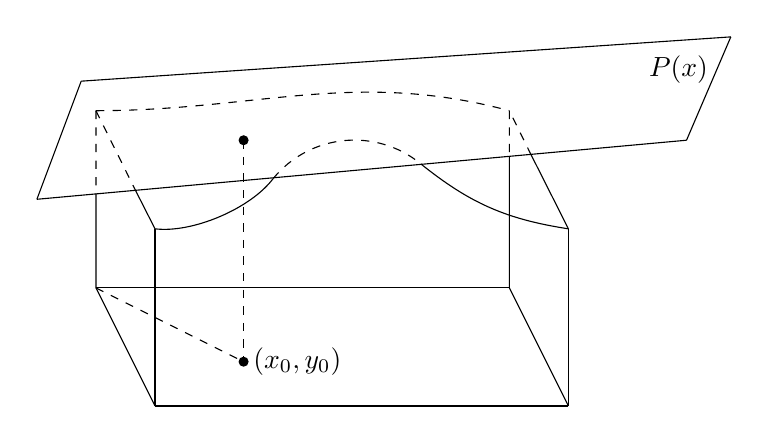
\begin{tikzpicture}[scale=0.75]
		\node [] (0) at (0, 0) {};
		\node [] (1) at (-1, 2) {};
		\node [] (2) at (6, 2) {};
		\node [] (3) at (7, 0) {};
		\node [] (4) at (-1, 5) {};
		\node [] (5) at (0, 3) {};
		\node [] (6) at (6, 5) {};
		\node [] (7) at (7, 3) {};
		\node [] (8) at (-2, 3.5) {};
		\node [] (9) at (9, 4.5) {};
		\node [] (10) at (-1.25, 5.5) {};
		\node [] (11) at (9.75, 6.25) {};
		\node [] (12) at (2, 3.85) {};
		\node [] (13) at (4.5, 4.1) {};
		\node [] (14) at (6.37, 4.25) {};
		\node [] (15) at (-0.3, 3.65) {};
		\draw [] (3.center) to (2.center);
		\draw [] (2.center) to (1.center);
		\draw [] (1.center) to (0.center);
		\draw [] (0.center) to (3.center);

		\draw (5.center) to (-0.33,3.65);
		\draw[dashed] (4.center) to (-0.33,3.65);
		

		\draw (1.center) to (-1,3.59);
		\draw [dashed] (4.center) to (-1,3.59); 
		
		
		\draw [] (5.center) to (0.center);
		
		\draw (2.center) to (6,4.22);
		\draw[dashed] (6.center) to (6,4.22);
%		\draw [] (6.center) to (2.center);
		
		
		\draw [] (7.center) to (3.center);
		\draw [] (10.center) to (8.center);
		\draw [] (10.center) to (11.center);
		\draw [] (11.center) to (9.center);
		\draw [] (9.center) to (8.center);
		\draw [, bend right, looseness=0.75] (5.center) to (12.center);
		\draw [dashed, bend left=45] (12.center) to (13.center);
		\draw [, bend right=15] (13.center) to (7.center);
		\draw [dashed, in=165, out=0] (4.center) to (6.center);
		\draw [] (7.center) to (14.center);
		\draw [dashed] (14.center) to (6.center);
		
		\draw (8.2,5.7) node [anchor=west]{$P(x)$};
		
		\draw[fill=black] (1.5,4.5) circle (0.075);
		\draw[fill=black] (1.5,0.75) circle (0.075);
		\draw[dashed] (1.center) to (1.5,0.75) node [anchor=west]{$\left( x_0,y_0\right)$};
		\draw[dashed] (1.5,4.5) to (1.5,0.75);
\end{tikzpicture}
\end{center}

\subsubsection*{Beispiel 8.5}
\begin{enumerate}[\indent a)]
\item Jede affin lineare Funktion $f(x)=Ax+b$, $x\in\R^n$, wobei $a:\R^n\to\R$ linear, $b$ $\in\R$ ist an jeder Stelle $x_0\in\R^n$ differenzierbar, mit $\mathop {df}\limits_{{x_0}} =A$ unabhängig von $x_0$, da
\[f\left( x \right) - f\left( {{x_0}} \right) - A\left( {x - {x_0}} \right) = 0\hspace{10mm}\forall x,{x_0} \in\R^n\]
\item Koordinatenfunktionen $x^i:\R^n\to\R$, $\left( x^1,x^2,\dots,x^n\right)\mapsto x^i$, $x^i(x)=x^i$. Dann ist $x^i$ differenzierbar an jeder Stelle $x_0\in\R^n$ mit
\[{\left. {d{x^i}} \right|_{x = {x_0}}} = \left( {0, \ldots ,0,1,0, \ldots ,0} \right)\]
Die Differentiale $dx^1,dx^2,\dots,dx^n$ bilden also an jeder Stelle $x_0\in\R^n$ eine Basis des Raumes $L\left( {\R^n:\R} \right):=\left\{ A:\R^n\to\R; A\text{ linear}\right\}$, wobei wir $A\in L\left( \R^n:\R\right)$ mit der Darstellung $A=\left( A_1,\dots,A_n\right)$ bzgl. der Standardbasis $\{ e_1,\dots,e_n\}$ der $\R^n$ identifizieren, und mit $A_i=A\left( e_i\right)$ \[d{x^i} = \left( {0, \ldots ,0,1,0, \ldots ,0} \right)\]\[\left( {d{x^i}\left( {{e_1}} \right),d{x^i}\left( {{e_2}} \right), \ldots ,d{x^i}\left( {{e_n}} \right)} \right)\]
Da $d{x^i}\left( {{e_j}} \right) = \left\{ {\begin{array}{*{20}{c}}
1&{i = j}\\
0&{i\not  = j}
\end{array}} \right.$ gilt, ist ${\left( {d{x^i}} \right)_{1 \le i \le n}}$ die duale Basis von $L\left( \R^n:\R\right)$ zur Standardbasis ${\left( {e_i} \right)_{1 \le i \le n}}$ des $\R^n$.
\item Jedes $f:\R\to\R\in C^1\left(\R\right)$ besitzt das Differential \[df\left( {{x_0}} \right) = \frac{{df}}{{dx}}\left( {{x_0}} \right)dx = f'\left( {{x_0}} \right)dx\] d.h. $f'\left(x_0\right)$ ist die Darstellung von $df\left(x_0\right)$ bezüglich der Basis $dx$ von $L\left(\R:\R\right)$
\item $f\left(x,y\right)=xe^y$, $\R^2\to\R$ ist an jeder Stelle $\left(x_0,y_0\right)\in\R^2$ differenzierbar und es gilt \[df\left( {{x_0},{y_0}} \right) = \left( {\frac{{\partial f}}{{\partial x}}\left( {{x_0},{y_0}} \right),\frac{{\partial f}}{{\partial y}}\left( {{x_0},{y_0}} \right)} \right) = \left( {{e^{{y_0}}},x{e^{{y_0}}}} \right)\] \[f\left( {x,y} \right) - f\left( {{x_0},{y_0}} \right) = \underbrace {f\left( {x,y} \right) - f\left( {{x_0},y} \right)}_ \swarrow  + f\left( {{x_0},y} \right) - f\left( {{x_0},{y_0}} \right)\] \[ = \frac{{\partial f}}{{\partial x}}\left( {\xi ,y} \right)\left( {x - {x_0}} \right) + \frac{{\partial f}}{{\partial y}}\left( {{x_0},\eta } \right)\left( {y - {y_0}} \right)\]
Nach dem Mittelwertsatz der Differentialrechnung, mit geeigneten Zwischenstellen $\xi=\xi (y)$ und $\eta$ \[ = \frac{{\partial f}}{{\partial x}}\left( {{x_0},{y_0}} \right)\left( {x - {x_0}} \right) + \frac{{\partial f}}{{\partial y}}\left( {{x_0},{y_0}} \right)\left( {y - {y_0}} \right) + R\left( {x,y} \right)\]
mit
\begin{align*}
 R\left( {x,y} \right) = &\left[ {\frac{{\partial f}}{{\partial x}}\left( {\xi ,y} \right) - \frac{{\partial f}}{{\partial x}}\left( {{x_0},{y_0}} \right)} \right]\left( {x - {x_0}} \right) \\
 + &\left[ {\frac{{\partial f}}{{\partial y}}\left( {{x_0},\eta } \right) - \frac{{\partial f}}{{\partial y}}\left( {{x_0},{y_0}} \right)} \right]\left( {y - {y_0}} \right)
\end{align*}
Wegen der Stetigkeit der Funktionen \[\frac{{\partial f}}{{\partial x}}\left( {x,y} \right) = {e^y}\hspace{5mm}\text{und}\hspace{5mm}\frac{{\partial f}}{{\partial y}}\left( {x,y} \right) = x{e^y}\] können wir den ``Fehler'' $R\left( x,y\right)$ leicht abschätzen \[\frac{{\abs{ {R\left( {x,y} \right)} }}}{{\abs{ {\left( {x,y} \right) - \left( {{x_0},{y_0}} \right)} }}} \le \sup_{\substack{\abs{ {\xi  - {x_0}} } < \abs{x - {x_0}} \\ \abs{\eta  - {y_0}} < \abs{y - y_0}}}{\left( {\abs{ {{e^y} - {e^{{y_0}}}} } + \abs{ {{x_0}} }\abs{ {{e^\eta } - {e^{{y_0}}}} }} \right)}\]
Für $\left( x,y\right)\to\left( x_0,y_0\right)$, $\left( x,y\right)\not=\left( x_0,y_0\right)$: d.h. es gilt \[\frac{{R\left( {x,y} \right)}}{{\abs{ {\left( {x,y} \right) - \left( {{x_0},{y_0}} \right)} }}} \to 0\]
d.h. es gilt \[\frac{{f\left( {x,y} \right) - f\left( {{x_0},{y_0}} \right) - \frac{{\partial f}}{{\partial x}}\left( {{x_0},{y_0}} \right)\left( {x - {x_0}} \right) - \frac{{\partial f}}{{\partial y}}\left( {{x_0},{y_0}} \right)\left( {y - {y_0}} \right)}}{{\abs{ {\left( {x,y} \right) - \left( {{x_0},{y_0}} \right)} }}}\mathop  \to \limits_{\left( {x,y} \right) \to \left( {{x_0},{y_0}} \right)} 0\]
 d.h. $f\left( x,y\right)$ ist in $(x_0, y_0)$ differenzierbar und
\[df\left( {{x_0},{y_0}} \right) = \left( {\frac{{\partial f}}{{\partial x}}\left( {{x_0},{y_0}} \right),\frac{{\partial f}}{{\partial y}}\left( {{x_0},{y_0}} \right)} \right)\]
\item Die Funktion \[f\left( {x,y} \right) = \left\{ {\begin{array}{*{20}{c}}
{\frac{{{x^3}y}}{{{x^2} + {y^2}}}}&{\left( {x,y} \right)\not  = \left( {0,0} \right)}\\
0&{\left( {x,y} \right) = \left( {0,0} \right)}
\end{array}} \right.\] ist in $\left( 0,0\right)$ differenzierbar. \\

Wir haben schon gesehen, dass $\frac{\partial f}{\partial x}\left( 0,0\right)=0$ und $\frac{\partial f}{\partial y}\left( 0,0\right)=0$. Dann gilt \[\frac{{\abs{ R }}}{{\abs{ {\left( {x,y} \right)} }}} = \frac{{\abs{ {f\left( {x,y} \right) - f\left( {0,0} \right) - \frac{{\partial f}}{{\partial x}}\left( {0,0} \right)\left( {x - 0} \right) - \frac{{\partial f}}{{\partial y}}\left( {0,0} \right)\left( {y - 0} \right)} }}}{{\abs{ {\left( {x - 0,y - 0} \right)} }}}\] \[ = \frac{{\abs{ {f\left( {x,y} \right) - 0 - 0 - 0} }}}{{\abs{ {\left( {x,y} \right)} }}} = \frac{{\abs{ {f\left( {x,y} \right)} }}}{{\abs{ {\left( {x,y} \right)} }}}\]
Zu untersuchen ist
\[\mathop {\lim }\limits_{\left( {x,y} \right) \to \left( {0,0} \right)}  \frac{{\abs{ {R\left( {\left( {x,y} \right),\left( {0,0} \right)} \right)} }}}{{\left( {x,y} \right) - \left( {0,0} \right)}} = \mathop {\lim }\limits_{\left( {x,y} \right) \to \left( {0,0} \right)} \frac{{\abs{ {f\left( {x,y} \right)} }}}{{\abs{ {\left( {x,y} \right)} }}}\]
Mittels Polarkoordinaten ist dies noch offensichtlicher
\[\mathop {\lim }\limits_{\left( {x,y} \right) \to \left( {0,0} \right)} \frac{{\abs{ {f\left( {x,y} \right)} }}}{{{x^2} + {y^2}}} = \mathop {\lim }\limits_{r \to 0} \frac{{{r^4}{{\cos }^3}\theta \sin \theta }}{{{r^2}}} = \mathop {\lim }\limits_{r \to 0} {r^2}{\cos ^3}\theta \sin \theta  = 0\] \[\Rightarrow f\text{ in }\left( 0,0\right)\text{ differenzierbar}\]
\end{enumerate}

\noindent Gibt es eine Beziehung zwischen dem Differential und den partiellen Ableitungen?

\subsubsection*{Bemerkung 8.6}

Sei $f:\Omega\to\R$, $\Omega\subset\R^n$ differenzierbar an der Stelle $x_0\in\Omega$. Dann existieren die partiellen Ableitungen $\frac{\partial f}{\partial x^i}\left( x_0\right)$, $i=1,\dots,n$ und dass Differential kann als \[{d_{{y_0}}}f = \left( {\frac{{\partial f}}{{\partial {x^1}}}\left( {{x_0}} \right), \ldots ,\frac{{\partial f}}{{\partial {x^n}}}\left( {{x_0}} \right)} \right)\] dargestellt werden.

\subsubsection*{Beweis}
Sei $f$ an der Stelle $x_0$ differenzierbar \[\Rightarrow f\left( {{x_0} + h{e_i}} \right) = f\left( {{x_0}} \right) + \left( {{d_{{x_0}}}f} \right)\left( {h{e_i}} \right) + R\left( {{x_0} + h{e_i},{x_0}} \right)\] wobei \[\mathop {\lim }\limits_{h \to 0} \frac{{R\left( {{x_0} + h{e_i},{x_0}} \right)}}{h} = \lim \frac{{f\left( {{x_0} + h{e_i}} \right) - f\left( {{x_0}} \right)\left( {{d_{{x_0}}}f\left( {h{e_i}} \right)} \right)}}{h} = 0\] \[ \Rightarrow \lim \frac{{f\left( {{x_0} + h{e_i}} \right) - f\left( {{x_0}} \right)}}{h} = \lim \frac{{h{d_{{x_0}}}f\left( {{e_i}} \right)}}{h} = {d_{{x_0}}}f\left( {{e_i}} \right)\] d.h. $\frac{\partial f}{\partial x^i}\left( x_0\right)$ existiert und $=d_{x_0}f\left( e_i\right)$. \\

Da $\left( dx^i\right)_{i=1,\dots,n}$ die zur $\left( e_j\right)_{1\leq j\leq n}$ duale Basis ist \[{d_{{x_0}}}f = \sum\limits_{i = 1}^n {\frac{{\partial f}}{{\partial {x^i}}}\left( {{x_0}} \right)d{x^i} = \left( {\frac{{\partial f}}{{\partial {x^1}}}\left( {{x_0}} \right),\frac{{\partial f}}{{\partial {x^2}}}\left( {{x_0}} \right), \ldots ,\frac{{\partial f}}{{\partial {x^n}}}\left( {{x_0}} \right)} \right)} \]

\subsubsection*{Beispiel}
Die Funktion \[f\left( {x,y} \right) = \left\{ {\begin{array}{*{20}{c}}
{\frac{{xy}}{{{x^2} + {y^2}}}}&{\left( {x,y} \right)\not  = \left( {0,0} \right)}\\
0&{\left( {x,y} \right) = \left( {0,0} \right)}
\end{array}} \right.\] ist in $\left( 0,0\right)$ nicht differenzierbar ($f$ ist  in $\left( 0,0\right)$ nicht stetig)

\subsubsection*{Satz 8.7}
Falls $f:\Omega\to\R$ in $x_0\in\Omega\subset\R$ differenzierbar ist, ist sie in $x_0$ auch stetig.

\subsubsection*{Beweis}
Folgt aus der Definition
\begin{definition}{8.8}
$f:\Omega\to\R$ heisst von der Klasse $C^1$, $\left( f\in C^1\left(\Omega\right)\right)$, falls $f$ an jeder Stelle $x_0\in\Omega$ und in jede Richtung $e_i$ partiell differenzierbar ist und die Funktionen $x\to\frac{\partial f}{\partial x^i}\left(x\right)$ für jedes $1\leq i\leq n$ auf $\Omega$ stetig sind.
\end{definition}
\subsubsection*{Satz 8.9}
Sei $f\in C^1\left(\Omega\right)$. Dann ist $f$ an jeder Stelle $x_0\in\Omega$ differenzierbar.

\subsubsection*{Beweis}
Für $n=3$ seien $x=\left( x^1,x^2,x^3\right)$, $x_0=\left( x_0^1,x_0^2,x_0^3\right)$. Dann ist
\begin{align*}
f\left( x \right) - f\left( {{x_0}} \right) = &\left\{ {f\left( {{x^1},{x^2},{x^3}} \right) - f\left( {{x^1},{x^2},x_0^3} \right)} \right\}\\
+ &\left\{ {f\left( {{x^1},{x^2},x_0^3} \right) - f\left( {{x^1},x_0^2,x_0^3} \right)} \right\}\\
+ &\left\{ {f\left( {{x^1},x_0^2,x_0^3} \right) - f\left( {x_0^1,x_0^2,x_0^3} \right)} \right\}
\end{align*}
Nach dem MWS der DR gilt: \[f\left( {{x^1},x_0^2,x_0^3} \right) - f\left( {x_0^1,x_0^2,x_0^3} \right) = \frac{{\partial f}}{{\partial {x^1}}}\left( {{\xi ^1},x_0^2,x_0^3} \right)\left( x^1-x_0^1\right)\]
wobei $\xi^1$ zwischen $x_0^1$ und $x^1$. Analog:
\[f\left( {{x^1},{x^2},x_0^3} \right) - f\left( {{x^1},x_0^2,x_0^3} \right) = \frac{{\partial f}}{{\partial {x^2}}}\left( {{x^1},{\xi ^2},x_0^3} \right)\left( {{x^2} - x_0^2} \right)\] wobei $\xi^2\in\left(x_0^2,x^2\right)$
und \[f\left( {{x^1},{x^2},{x^3}} \right) - f\left( {{x^1},{x^2},x_0^3} \right) = \frac{{\partial f}}{{\partial {x^3}}}\left( {{x^1},{x^2},{\xi ^3}} \right)\left( {{x^3} - x_0^3} \right)\]
Eingesetzt in den Ausdruck für $f(x)-f(x_0)$ ergibt:
\begin{align*}
f\left( x \right) - f\left( {{x_0}} \right) = &\frac{{\partial f}}{{\partial {x^1}}}\left( {{\xi ^1},x_0^2,x_0^3} \right)\left( {{x^1} - x_0^1} \right)\\
+ &\frac{{\partial f}}{{\partial {x^2}}}\left( {{x^1},{\xi ^2},x_0^3} \right)\left( {{x^2} - x_0^2} \right)\\ + &\frac{{\partial f}}{{\partial {x^3}}}\left( {{x^1},{x^2},{\xi ^3}} \right)\left( {{x^3} - x_0^3} \right)
\end{align*}
Also
\[f\left( x \right) - f\left( {{x_0}} \right) = \sum\limits_{i = 1}^3 {\frac{{\partial f}}{{\partial {x^1}}}\left( {x_0^1,x_0^2,x_0^3} \right)\left( {{x^i} - x_0^i} \right)}  + R\left( {{x_0},x} \right)\]
Wobei
\begin{align*}
R\left( {{x_0},x} \right) = &\left( {\frac{{\partial f}}{{\partial {x^1}}}\left( {{\xi ^1},x_0^2,x_0^3} \right) - \frac{{\partial f}}{{\partial {x^1}}}\left( {x_0^1,x_0^2,x_0^3} \right)} \right)\left( {{x^1} - x_0^1} \right)\\
 + &\left( {\frac{{\partial f}}{{\partial {x^2}}}\left( {{x^1},{\xi ^2},x_0^3} \right) - \frac{{\partial f}}{{\partial {x^2}}}\left( {x_0^1,x_0^2,x_0^3} \right)} \right)\left( {{x^2} - x_0^2} \right)\\
 + &\left( {\frac{{\partial f}}{{\partial {x^3}}}\left( {{x^1},{x^2},{\xi ^3}} \right) - \frac{{\partial f}}{{\partial {x^3}}}\left( {x_0^1,x_0^2,x_0^3} \right)} \right)\left( {{x^3} - x_0^3} \right)
\end{align*}
Also
\[\abs{ {R\left( {x,{x_0}} \right)} } < \abs{ {x - {x_0}} }\underbrace {\left\{ {\abs{ {\left(  \ldots  \right)} } + \abs{ {\left(  \ldots  \right)} } + \abs{ {\left(  \ldots  \right)} }} \right\}}_{\scriptstyle \to 0{\text{ mit }}x \to {x_0}\hfill\atop
\scriptstyle{\text{weil }}\frac{{\partial f}}{{\partial {x^i}}}{\text{ stetig sind}}\hfill}\]
Also ist $\lim\frac{R\left( x,x_0\right)}{\left( x-x_0\right)}=0$ und $f(x)$ ist differenzierbar.

\subsubsection*{Beispiel 8.10}
Polynome auf $\R^n$ sind von der Klasse $C^1$. Für jeden Multiindex $\alpha=\left(\alpha_0,\dots , \alpha_n\right)\in\N^n$ definieren wir die Monomialfunktion \[{x^\alpha }: = {\left( {{x^0}} \right)^{{\alpha _0}}}{\left( {{x^1}} \right)^{{\alpha _1}}} \ldots {\left( {{x^n}} \right)^{{\alpha _n}}}\] Ein Polynom von Grad $\leq N$ ist dann gegeben durch \[p(x) = \sum\limits_{\abs{ \alpha  } \le N} {{a_\alpha }{x^\alpha }} \] wobei $\abs{ \alpha  } = {\alpha _0} +  \ldots  + {\alpha _n}$
\todo[inline]{Pages 135.1 - 135.2 are a Zusammenfassung, not sure if needed to be included}
\section{Differentiationsregeln}
Ganz analog zum eindimensionalen Fall gelten folgende Differentiationsregeln

\subsubsection*{Satz 8.11}
Sei $\Omega\subset\R^n$, sowie $f,g:\Omega\to\R$ an der Stelle $x_0\in\Omega$ differenzierbar. Dann gilt \begin{enumerate}
\item $d\left( {f + g} \right)\left( {{x_0}} \right) = df\left( {{x_0}} \right) + dg\left( {{x_0}} \right)$
\item $d\left( {fg} \right)\left( {{x_0}} \right) = g\left( {{x_0}} \right)df\left( {{x_0}} \right) + f\left( {{x_0}} \right)dg\left( {{x_0}} \right)$
\item Falls $g\left( x_0\right)\not=0$ \[d\left( {\frac{f}{g}} \right)\left( {{x_0}} \right) = \frac{{g\left( {{x_0}} \right)df\left( {{x_0}} \right) - f\left( {{x_0}} \right)dg\left( {{x_0}} \right)}}{{{{\left( {g\left( {{x_0}} \right)} \right)}^2}}}\]
\end{enumerate}
Beweis ist der Selbe wie im eindimensionalen Fall. Für die Kettenregel gibt es mehrere Variationen

\subsubsection*{Satz 8.12 (Kettenregel, 1. Version)}
Sei $g:\Omega\to\R$ in $x_0\in\Omega\subset\R^n$ differenzierbar, sowie $f:\R\to\R$ an der Stelle $g\left( x_0\right)\in\R$ differenzierbar. Dann gilt \[d\left( {f \circ g} \right)\left( {{x_0}} \right) = f'\left( {g\left( {{x_0}} \right)} \right) \cdot dg\left( {{x_0}} \right)\]

\begin{center}
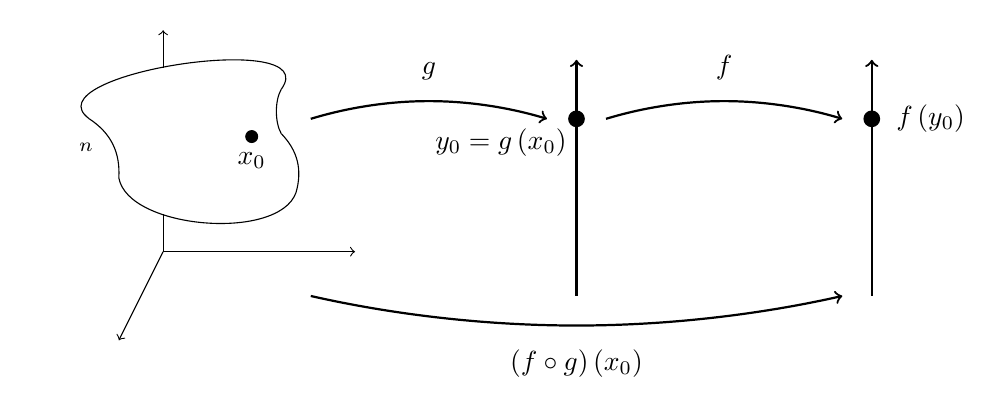
\begin{tikzpicture}[scale=0.75]
\draw[thick,->] (5,0) -- (5,4) node[anchor=south]{$\R$};
\draw[thick,->] (5.5,3) parabola bend(7.5,3.3)(9.5,3);
\draw(7.5,3.5) node[anchor=south] {$f$};

\draw[thick,->] (10,0) -- (10,4);
\draw[thick,->] (0.5,3) parabola bend(2.5,3.3)(4.5,3);
\draw(2.5,3.5) node[anchor=south] {$g$};

\draw[thick,->] (0.5,0) parabola bend(5,-0.5)(9.5,0);
\draw(5,-0.75) node[anchor=north] {$\left( f\circ g\right) \left( x_0\right)$};

\node[circle,fill=black,inner sep=0.75mm] (a) at (10,3) {};
\node[circle,fill=black,inner sep=0.75mm] (a) at (5,3) {};

\draw(10.25,3) node[anchor=west] {$f\left( y_0\right)$};
\draw(5,3) node[anchor=north east] {$y_0=g\left( x_0\right)$};

\draw(-3,2.75) node[anchor=north east] {$\R^n$};



		\node [] (0) at (-3.25, 3) {};
		\node [] (1) at (0, 3.5) {};
		\node [] (2) at (0, 2.75) {};
		\node [] (3) at (0.25, 1.75) {};
		\node [] (4) at (-2.75, 2) {};
		\draw [bend left=135] (0.center) to (1.center);
		\draw [bend right, looseness=0.75] (1.center) to (2.center);
		\draw [bend left] (2.center) to (3.center);
		\draw [bend left=75, looseness=0.75] (3.center) to (4.center);
		\draw [bend left] (0.center) to (4.center);
\draw[fill=black] (-0.5,2.7) circle (0.1);
\draw[anchor=north] (-0.5,2.6) node {$x_0$};

\draw[->] (-2,0.75) -- (1.25,0.75);
\draw[->] (-2,0.75) -- (-2.75,-0.75);
\draw[] (-2,0.75) -- (-2,1.385);
\draw[->] (-2,3.865) -- (-2,4.5);
\end{tikzpicture}
\end{center}

\subsubsection*{Beweis}
Sei $g$ an der Stelle $x_0$ differenzierbar
\[ \Rightarrow g\left( x \right) - g\left( {{x_0}} \right)\mathop  = \limits^A dg\left( {{x_0}} \right)\left( {x - {x_0}} \right) + {R_g}\left( {x - {x_0}} \right)\]
mit \[\frac{{{R_g}\left( {x - {x_0}} \right)}}{{\left( {x - {x_0}} \right)}}\mathop  \to \limits_{x \to {x_0}} 0 \Rightarrow \frac{{g\left( x \right) - g\left( {{x_0}} \right)}}{{\abs{ {x - {x_0}} }}}\mathop  \le \limits^B C = \max \left[ {\frac{{\partial g}}{{\partial {x^i}}}\left( {{x_0}} \right)} \right]\] $f$ in $g\left( x_0\right)$ differenzierbar
\[f\left( {g\left( x \right)} \right) - f\left( {g\left( {{x_0}} \right)} \right)\mathop  = \limits^C f'\left( {g\left( {{x_0}} \right)} \right)\left[ {g(x) - g\left( {{x_0}} \right)} \right] + {R_f}\left( {g\left( x \right),g\left( {{x_0}} \right)} \right)\]
Woraus folgt:
\begin{align*}
f\left( {g\left( x \right)} \right) - f\left( {g\left( {{x_0}} \right)} \right) = & f'\left( {g\left( {{x_0}} \right)} \right)\left[ {dg\left( {{x_0}} \right)\left( {x - {x_0}} \right) + {R_g}\left( {x,{x_0}} \right)} \right]\\ + & {R_f}\left( {g\left( {{x_0}} \right),g\left( x \right)} \right)
\end{align*}

Aus B folgt:
\[\frac{{{R_f}\left( {g\left( {{x_0}} \right),g\left( x \right)} \right)}}{{x - {x_0}}} = \underbrace {\underbrace {\frac{{{R_f}\left( {g\left( {{x_0}} \right) - g\left( x \right)} \right)}}{{\abs{ {g\left( x \right) - g\left( {{x_0}} \right)} }}}}_{\begin{array}{*{20}{c}}
 \downarrow \\
0
\end{array}} \cdot \underbrace {\frac{{\abs{ {g\left( x \right) - g\left( {{x_0}} \right)} }}}{{\abs{ {x - {x_0}} }}}}_{\mathop  \le \limits^B C}}_{\begin{array}{*{20}{c}}
 \downarrow \\
0
\end{array}}\]
d.h.
\[f\left( {g\left( x \right)} \right) - f\left( {g\left( {{x_0}} \right)} \right) = \left( {f'\left( {g\left( {{x_0}} \right)} \right) \cdot dg\left( {{x_0}} \right)} \right)\left( {x - {x_0}} \right) + {R_{f \circ g}}\left( {x,{x_0}} \right)\]
wobei
\[{R_{f \circ g}}\left( {x,{x_0}} \right) = f'\left( {g\left( {{x_0}} \right)} \right){R_g}\left( {x,{x_0}} \right) + {R_f}\left( {g\left( {{x_0}} \right),g\left( x \right)} \right)\]
und
\[\frac{{{R_{f \circ g}}\left( {x,{x_0}} \right)}}{{x - {x_0}}} = \underbrace {f'\left( {g\left( {{x_0}} \right)} \right)\frac{{{R_g}\left( {x,{x_0}} \right)}}{{\left( {x - {x_0}} \right)}}}_{ \downarrow 0} + \underbrace {\frac{{{R_f}\left( {g\left( {{x_0}} \right),g\left( x \right)} \right)}}{{x - {x_0}}}}_{ \downarrow 0}\]

\subsubsection*{Beispiel 8.13}
Sei $h:\R^2\to\R$ \[h(x,y)=e^{xy}\] $h= f\circ g$ wobei $g(x,y)=xy$, $f(t)=e^t$. Dann ist einerseits \[dh\left( {x,y} \right) = \left( {\frac{{\partial h}}{{\partial x}},\frac{{\partial h}}{{\partial y}}} \right) = \left( {y{e^{xy}},x{e^{xy}}} \right)\] anderseits nach Kettenregel
\[dh\left( {x,y} \right) = d\left( {f \circ g} \right)' = f'\left( {g\left( {x,y} \right)} \right) \cdot dg\left( {x,y} \right) = {e^{xy}} \cdot \left( {y,x} \right) = \left( {y{e^{xy}},x{e^{xy}}} \right)\]
Für die nächste Kettenregel führen wir folgende Definition ein:

\begin{definition}{8.14}
Sei $\Omega \subset\R$ und $f=\left( f_1,\dots,f_n\right):\Omega\to\R^n$ eine Abbildung. Dann ist $f$ an der Stelle $x_0\in\R$ differenzierbar, falls jede Komponentenfunktion $f_i$ an der Stelle $x_0$ differenzierbar ist. Wir definieren in diesem Fall \[f'\left( {{x_0}} \right): = \left( {{f_1}'\left( {{x_0}} \right),{f_2}'\left( {{x_0}} \right), \ldots ,{f_n}'\left( {{x_0}} \right)} \right)\]
\end{definition}

\subsubsection*{Bemerkung 8.15}
$f'\left( x_0\right)$ kann als Geschwindigkeitsvektor im Punkt $f\left( x_0\right)$ aufgefasst werden.

\subsubsection*{Satz 8.16 (Kettenregel, 2. Version)}
Sei $\Omega\subset\R^n,I\subset\R$. Sei $g:I\to\Omega$, $t\to\left( g_1(t), g_2(t),\dots, g_n(t)\right)$, an der Stelle $t_0\in I$ differenzierbar sowie $f:\Omega\to\R$ an der Stelle $g\left( t_0\right)$ differenzierbar. Dann gilt:
\[\frac{d}{{dt}}\left( {f \circ g} \right)\left( {{t_0}} \right) = df\left( {g\left( {{t_0}} \right)} \right) \cdot g'\left( {{t_0}} \right)\]
\begin{align*}
d\left( {f \circ g} \right)\left( {{t_0}} \right) =& df\left( {g\left( {{t_0}} \right)} \right) \cdot dg\left( {{t_0}} \right)\\
 =& \frac{{\partial f}}{{\partial {x^1}}}\left( {g\left( {{t_0}} \right)} \right) \cdot \frac{{d{g_1}}}{{dt}}\left( {{t_0}} \right) + \frac{{\partial f}}{{\partial {x^2}}}\left( {g\left( {{t_0}} \right)} \right) \cdot \frac{{d{g_2}}}{{dt}}\left( {{t_0}} \right)\\ & + \ldots  + \frac{{\partial f}}{{\partial {x^n}}}\left( {g\left( {{t_0}} \right)} \right) \cdot \frac{{d{g_n}}}{{dt}}\left( {{t_0}} \right)
\end{align*}


\begin{center}
\begin{tikzpicture}[scale=0.9]


\node [] (0) at (1, 3) {};
\node [] (1) at (2.75, 1.75) {};
\node [] (2) at (-1, 1.75) {};
\node [] (3) at (1.5, -0.5) {};
\node [] (4) at (-0.25, 0.75) {};
\node [] (5) at (2.25, 2) {};

\draw [ bend left=75, looseness=1.25] (0.center) to (1.center);
\draw [bend right=75, looseness=1.25] (2.center) to (3.center);
\draw [in=-135, out=45, looseness=1.50] (2.center) to (0.center);
\draw [in=-135, out=30] (3.center) to (1.center);
\draw [in=-135, out=45, looseness=1.25] (4.center) to (5.center);

\draw[->](0.5,1.25)--(1.2,1.7);
\draw[fill=black] (0.5,1.25) circle (0.05);

\draw (0.5,1.25) node[anchor=north]{$g(t_0)$};
\draw (1.2,1.7) node[anchor=south]{$g'(t_0)$};

\draw[->] (0,2.37)--(0,4) node [anchor=south]{$\R^n$};
\draw[->] (2.25,0.8)--(4,0.8);
\draw[->] (-0.5,-0.3)--(-1,-1);


\draw[->](-5,0) -- (-5,4) node [anchor=south]{$\R$};
\draw[fill=black] (-5,2) circle (0.05) node [anchor=west]{$t_0$};

\draw [bend left=15,->] (-4,3) to (-1,3);
\draw (-2.5,3.2)node [anchor=south]{$g$};

\draw [bend left=15,->] (4,3) to (7,3);
\draw (5.5,3.2)node [anchor=south]{$f$};

\draw[->](8,0) -- (8,4);
\draw[fill=black] (8,2) circle (0.05) node [anchor=east]{$\left( f\circ g\right)(t)$};
\end{tikzpicture}

\begin{tikzpicture}[scale=1]



\node [] (4) at (-0.25, 0.75) {};
\node [] (5) at (2.25, 2) {};


\draw [in=-135, out=45, looseness=1.25] (4.center) to (5.center) node [anchor=west]{$g(t)$};

\draw[->](0.5,1.25)--(1.2,1.7);
\draw[fill=black] (0.5,1.25) circle (0.05);

\draw (0.5,1.25) node[anchor=north]{$g(t_0)$};
\draw (1.2,1.7) node[anchor=south]{$g'(t_0)$};

\draw[bend left=20] (-3,1.25) to (0.5,1.25); 
\draw (-1.25,1.6) node [anchor=south]{$g$};

\draw[->](-3,0)--(-3,3) node [anchor=west]{$t$};
\draw[fill=black] (-3,1.25) circle (0.05) node[anchor=east]{$t_0$};

\draw[thick] (-2.9,2) --(-3.1,2);
\draw[thick] (-2.9,2.0125) --(-2.9,1.9);
\draw[thick] (-3.1,2.0125) --(-3.1,1.9);

\draw[thick] (-2.9,0.5) --(-3.1,0.5);
\draw[thick] (-2.9,0.4875) --(-2.9,0.6);
\draw[thick] (-3.1,0.4875) --(-3.1,0.6);

\draw(-2.5,0.8) node  [anchor=east]{$I$};
\end{tikzpicture}
\end{center}


\subsubsection*{Beispiel 8.17}
Die vier Grundrechenarten sind differenzierbare Funktionen von zwei Variablen. Insbesondere gilt:
\begin{itemize}
\item $a:\R^2\to\R$, $\left( x,y\right) \to x+y$ \[da\left( {x,y} \right) = \left( {\frac{{\partial a}}{{\partial x}},\frac{{\partial a}}{{\partial y}}} \right) = \left( {1,1} \right)\]
\item $m:\R^2\to \R$, $\left( x,y\right) \to x\cdot y$ \[dm\left( {x,y} \right) = \left( {y,x} \right)\]
\end{itemize}
Setzt man diese beiden Funktionen in die obige Kettenregel ein, so erhält man die aus Analysis I bekannte Summen- und Produktregel:
\[g:\R\to\R^2, t\to \left( g_1(t),g_2(t)\right)\]
\[\frac{d}{{dt}}\left( {{g_1} + {g_2}} \right) = \frac{d}{{dt}}\left( {a \circ g} \right) = \left( {1,1} \right) \cdot \left( {\frac{{d{g_1}}}{{dt}},\frac{{d{g_2}}}{{dt}}} \right) = 1\cdot \frac{{d{g_1}}}{{dt}} + 1\cdot \frac{{d{g_2}}}{{dt}}\]
und
\begin{align*}
\frac{d}{{dt}}\left( {{g_1} \cdot {g_2}} \right) = \frac{d}{{dt}}\left( {m \circ g} \right) = &\left( {\left( {dm} \right)\left( {g(t)} \right)} \right) \cdot \left( {\frac{{dg}}{{dt}}} \right)\\
= &\left( {{g_2}\left( t \right),{g_1}\left( t \right)} \right) \cdot \left( {\frac{{d{g_1}}}{{dt}},\frac{{d{g_2}}}{{dt}}} \right)\\
= &\frac{{d{g_1}}}{{dt}} \cdot {g_2}\left( t \right) + \frac{{d{g_2}}}{{dt}} \cdot {g_1}\left( t \right)
\end{align*}

\subsubsection*{Beispiel 8.18}
Sei $f:\Omega\to\R$ differenzierbar an der Stelle $x_0\in\Omega$ und sei $e\in\R^n\setminus\{ 0\}$; mit $\abs{ e}=1$. Betrachte die Gerade $g(t)=x_0+te$, $t\in\R$ durch $x_0$ mit Richtungsvektor

\begin{figure}[H]
\begin{minipage}[b]{0.45\linewidth}

\begin{center}
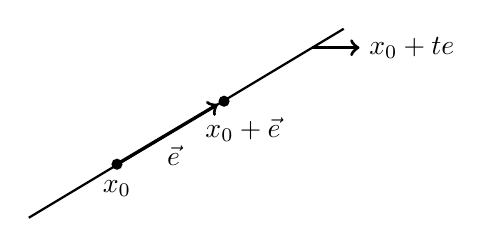
\begin{tikzpicture}[scale=0.8]
\draw[thick] (0,0) -- (5,3) ;

\node[circle,fill=black,inner sep=0.5mm] (a) at (1.4,0.85) {};
\draw (1.4,0.75) node[anchor=north] {$x_0$};
\draw[very thick,->] (1.4,0.85) -- (3,1.8) ;

\node[circle,fill=black,inner sep=0.5mm] (a) at (3.1,1.85) {};
\draw (3.4,1.75) node[anchor=north] {$x_0+\vec e$};
\draw (2.3,1.3) node[anchor=north] {$\vec e$};

\draw[very thick,->] (4.5,2.7) -- (5.25,2.7) ;
\draw (5.25,2.7) node[anchor=west] {$x_0+te$};
\end{tikzpicture}
\end{center}

\end{minipage}
\hspace{0.5cm}
\begin{minipage}[b]{0.45\linewidth}

\centering
\[\frac{dg}{dt}\left( t_0\right)=\R\hspace{5mm}\forall t_0\in\R\]
\begin{align*}
g:\R&\to\R^2\\
t&\mapsto x_0+te
\end{align*}

\end{minipage}
\end{figure}


Dann ist die Funktion $f\circ g$ in einer Umgebung von $t_0=0$ definiert und nach Kettenregel $f\circ g$ an der Stelle $t_0=0$ differenzierbar mit
\[\frac{d}{{dt}}\left( {f \circ g} \right)\left( 0 \right) = df\left( {g\left( 0 \right)} \right)\frac{{dg}}{{dt}}\left( 0 \right) = df\left( {{x_0}} \right)\left( e \right) = \sum\limits_{i = 1}^n {\frac{{\partial f}}{{\partial {x^i}}}\left( {{x_0}} \right) \cdot {e^i}} \]
$e=\left( e^1,\dots, e^n\right) $ und wird Richtungsableitung von $f$ in Richtung $e$ genannt; $\partial_ef\left( x_0\right)$ bezeichnet. Insbesondere gilt für $e=e_i$
\[{\partial _{{e_i}}}f\left( {{x_0}} \right) = \frac{{\partial f}}{{\partial {x^i}}}\left( {{x_0}} \right) = df\left( {{x_0}} \right)\left( {{e_i}} \right)\]
Geometrisch ist die Richtungsableitung von $f$ in Richtung $e$ genau die Steigung der Tangente zur Schnittkurve, falls wir den Graph von $f$ mit einer zur $xy$-Ebene senkrechten Ebene durch $x_0+te$ scheiden.
\missingfigure{page 144, middle. STARTED; CAN'T FULLY UNDERSTAND THE DRAWING DUE TO LINES BEING FADED ON THE PDF}
%\begin{tikzpicture}
%\node [] (0) at (0, 0) {};
%\node [] (1) at (0, 6) {};
%\node [] (2) at (8, 0) {};
%\node [] (3) at (3, 2) {};
%\node [] (4) at (1.5, 0) {};
%\node [] (5) at (7, 1.75) {};
%\node [] (6) at (7, 5) {};
%\node [] (7) at (1.5, 4) {};
%\node [] (8) at (1.5, 5) {};
%\node [] (9) at (7, 6) {};
%\node [] (10) at (7, 9) {};
%\node [] (11) at (1.5, 8) {};
%\draw [->] (0.center) to (1.center);
%\draw [->] (0.center) to (2.center);
%\draw [->] (0.center) to (3.center);
%\draw [] (4.center) to (5.center);
%\draw [] (5.center) to (6.center);
%\draw [] (4.center) to (7.center);
%\draw [] (8.center) to (11.center);
%\draw [] (11.center) to (10.center);
%\draw [] (10.center) to (9.center);
%\draw [, in=-150, out=30, looseness=1.50] (8.center) to (9.center);
%\draw [, in=-150, out=30, looseness=1.50] (7.center) to (6.center);
%
%\end{tikzpicture}
Um den Mittelwertsatz der DR zu verallgemeinern, benützen wir folgende Begriffe:
\begin{definition}{8.19}
Eine Menge $K\subset \R^n$ ist genau dann konvex, falls für jedes Paar von Punkten $x,y\in K$ die Menge $K$ auch das Segment \[\left( 1-t\right) x+ty\hspace{10mm} t\in\lbrack 0,y\rbrack\] mit Endpunkten $x,y$ enthält
\begin{multicols}{2}
\begin{center}
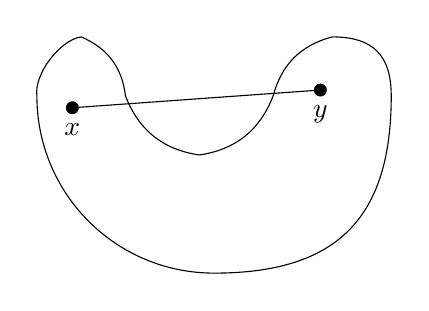
\begin{tikzpicture}[scale=0.75]
\node [] (0) at (1, 1) {};
\node [] (1) at (2, 2) {};
\node [] (2) at (3, 1) {};
\node [] (3) at (0, -2) {};
\node [] (4) at (-3, 1) {};
\node [] (5) at (-2.25, 2) {};
\node [] (6) at (-1.5, 1) {};
\node [] (7) at (-0.25, 0) {};

\draw [bend right=45] (4.center) to (3.center);
\draw [bend right=45, looseness=1.25] (3.center) to (2.center);
\draw [bend right=45, looseness=1.25] (2.center) to (1.center);
\draw [bend right] (1.center) to (0.center);
\draw [bend left] (0.center) to (7.center);
\draw [bend left] (7.center) to (6.center);
\draw [bend right] (6.center) to (5.center);
\draw [bend right=45, looseness=0.75] (5.center) to (4.center);

\draw[fill=black] (1.8,1.1) circle (0.1);
\draw[fill=black] (-2.4,0.8) circle (0.1);

\draw(-2.4,0.8) --(1.8,1.1);

\draw[](-2.4,0.7) node[anchor=north]{$x$};
\draw[](1.8,1.0) node[anchor=north]{$y$};
\end{tikzpicture}
\end{center}
\columnbreak
\begin{center}
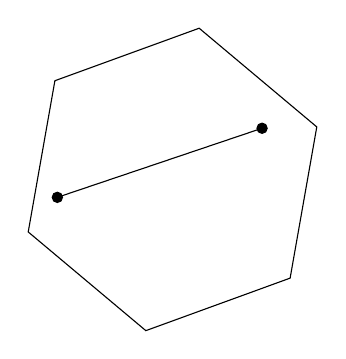
\begin{tikzpicture}[scale=0.65]
    \begin{scope}[rotate=320]
        \draw (0:3cm) \foreach \x in {60,120,...,359} {
                -- (\x:3cm)
            }-- cycle (90:3cm) ;
           \end{scope}
\draw (-2.25,-0.35) -- (1.75,1);
\draw[fill=black] (-2.25,-0.35) circle (0.1);
\draw[fill=black] (1.75,1) circle (0.1);

\end{tikzpicture}
\end{center}
\end{multicols}
\begin{multicols}{2}
\begin{center}
Nicht Konvex
\end{center}
\columnbreak
\begin{center}
Konvex
\end{center}
\end{multicols}
\end{definition}
\subsubsection*{Satz 8.20}
Sei $\Omega\subset\R^n$ konvex $f:\Omega\to\R$ differenzierbar, $x_0,x_1\in\Omega$ sowie ${x_t:=\left( 1-t\right) x_0+tx_1}$ mit ${t \in [0,1]}$. Dann gibt es $\vartheta\in\lbrack 0,1\rbrack$ mit \[f\left( {{x_1}} \right) - f\left( {{x_0}} \right) = df\left( {{x_{i\vartheta }}} \right)\left( {{x_1} - {x_0}} \right)\]

\subsubsection*{Beweis}
Sei $g\left( t\right) = \left( 1-t\right) x_0+tx_1=x_t$. Dann ist $t\to \left( f\circ g\right)(t)$ auf $\left[ 0,1\right]$ stetig und in $\left( 0,1\right)$ differenzierbar. Also gibt es $\vartheta\in\left( 0,1\right)$ mit (nach MWS der DR einer Variable) \[f\left( {{x_i}} \right) - f\left( {{x_0}} \right) = \left( {f \circ g} \right)(1) - \left( {f \circ g} \right)(0) = \left( {f \circ g} \right)'\left( \vartheta  \right)\left( {1 - 0} \right)\] Nun ist \[\left( {f \circ g} \right)'\left( \vartheta  \right) = df\left( {g\left( \vartheta  \right) \cdot \frac{{dg}}{{dt}}\left( \vartheta  \right)} \right)\] \todo{Is the formula done or does it continue on a new line, page 146 top}
%\[\left( {df} \right)\left( {{x_\vartheta }} \right)\left( { - {x_0} + {x_1}} \right)\]
Die Kettenregel wird auch abgewandelt um Integrale mit Parametern zu studieren. Ein Beispiel davon ist:

\subsubsection*{Beispiel}
Sei $h:\R^2\to\R$, $\left( s,t\right)\to h\left(s,t \right)$. Wir nehmen an, $h$ ist stetig, $\frac{\partial h}{\partial t}$ existiert und ist auf ganz $\R^2$ stetig. Sei
\[u(t) = \int\limits_a^{b(t)} {h(s,t)ds} {\text{, }}b(t) \in C^1\left( \R \right){\text{, }}a \in\R\]

\subsubsection*{Satz 8.21}
Sei $h(s,t)$ eine stetige differenzierbare Funktion von zwei Variablen und $b(t)$ differenzierbare Funktion einer Variable. Dann ist die Funktion \[u(t): = \int\limits_a^{b(t)} {h(s,t)ds} \] wo definiert, differenzierbar mit der Ableitung \[u'(t): = h\left( {b(t),t} \right) \cdot b'(t) + \int\limits_a^{b(t)} {\frac{{\partial h}}{{\partial t}}\left( {s,t} \right)ds} \]
\subsubsection*{Korollar 8.22}
Sei $h=h\left( s,t\right) :\R^2\to\R$ stetig, und $\frac{\partial h}{\partial t}$ existiert und auf ganz $\R^2$ stetig. Sei \[u(t) = \int\limits_0^t {h\left( {s,t} \right)ds} \] Dann \[u(t) \in C^1\left( \R\right)\text{ und }u'(t) = h\left( {t,t} \right) + \int\limits_0^t {\frac{{\partial h}}{{\partial t}}\left( {s,t} \right)ds} \]

\subsubsection*{Beweis}
Setze $b(t)=t$, $a=0$ in Satz 8.21.

\subsubsection*{Korollar 8.23}
Sei $h:\R^2\to\R$ eine stetige Funktion mit stetiger partieller Ableitung $\frac{\partial h}{\partial t}$. Dann ist die Funktion \[u(t): = \int\limits_a^b {h(s,t)ds} \] differenzierbar mit Ableitung \[u'(t): = \int\limits_a^b {\frac{{\partial h}}{{\partial t}}(s,t)ds} \]

\subsubsection*{Beweis}
Setze $b(t)=b$, in Satz 8.20

\subsubsection*{Bemerkung 8.24}
Mit Korollar 8.23 kann man bestimmte Integrale berechnen, auch wenn die dazugehörigen unbestimmten Integrale nicht elementar darstellbar sind
\subsubsection*{Beispiel 8.25}
Berechne das Integral \[\int\limits_0^1 {\frac{{{x^5} - 1}}{{\log x}}} dx\] Sei \[u\left( \alpha  \right): = \int\limits_0^1 {\frac{{{x^\alpha } - 1}}{{\log x}}dx} \] Für $\alpha \geq 0$ erfüllt $u\left(\alpha\right)$ die Voraussetzungen des Satzes. Wir berechnen \[u'\left( \alpha  \right) = \int\limits_0^1 {\frac{\partial }{{\partial \alpha }}\left( {\frac{{{x^\alpha } - 1}}{{\log x}}} \right)dx}  = \int\limits_0^1 {\frac{{{x^\alpha }\log x}}{{\log x}}dx = \int\limits_0^1 {{x^\alpha }dx}  = \left. {\frac{{{x^{\alpha  + 1}}}}{{\alpha  + 1}}} \right|_0^{x = 1} = } \frac{1}{{\alpha  + 1}}\]
Daraus folgt aus dem fundamentalen Satz der Integralrechnung \[u\left( \alpha  \right) = \int {u'\left( \alpha  \right)d\alpha  = \int {\frac{{d\alpha }}{{\alpha  + 1}} = \log \left( {\alpha  + 1} \right)} }  + C\]
Für eine noch zu bestimmende Konstante $C$. Aber
\[u\left( 0 \right) = \int\limits_0^1 {0dx = 0 \Rightarrow C = 0} \]
\[ \Rightarrow \int\limits_0^1 {\frac{{{x^\alpha } - 1}}{{\log x}}dx = \log \left( {\alpha  + 1} \right)} \]
\[ \Rightarrow \int\limits_0^1 {\frac{{{x^5} - 1}}{{\log x}}dx = \log 6} \]

\subsubsection*{Beweis Satz 8.21 (Idee)}
Sei \[f\left( {x,y} \right) = \int\limits_a^x {h\left( {s,y} \right)ds}:\R^2\to\R \]
\[g\left( t \right) = \left( {\begin{array}{*{20}{c}}
{b\left( t \right)}\\
t
\end{array}} \right):\R\to\R^2\text{, }g'\left( t \right) = \left( {\begin{array}{*{20}{c}}
{b'\left( t \right)}\\
1
\end{array}} \right)\]
Dann \[u(t) = \left( {f \circ g} \right)(t) = f\left( {b(t),t} \right) = \int\limits_a^{b(t)} {h(s,t)ds} \]
Nach dem Hauptsatz der Integralrechnung $f$ ist nach $x$ partielle differenzierbar und $\frac{\partial f}{\partial x}=h(x,y)$. Man muss zeigen, dass $f$ ist nach $y$ partiell differenzierbar mit \[\frac{{\partial f}}{{\partial y}}(x,y) = \int\limits_a^x {\frac{{\partial h(s,y)}}{{\partial x}}ds} \]
Dann ergibt die Kettenregel
\begin{align*}
u'(t) = &\frac{d}{{dt}}\left( {f \circ g} \right)(t) = \left( {\frac{{\partial f}}{{\partial x}}\left( {g(t)} \right),\frac{{\partial f}}{{\partial y}}\left( {g(t)} \right)} \right) \cdot \frac{{dg}}{{dt}}\\
= &\left( {h\left( {b(t),t} \right),\left( {\int\limits_a^x {\frac{{\partial h(s,y)}}{{\partial y}}ds} } \right)h\left( {b(t),t} \right)} \right)\left( {\begin{array}{*{20}{c}}
{b'(t)}\\
1
\end{array}} \right)\\
= &\left( {h\left( {b(t),t} \right),\int\limits_a^{b(t)} {\frac{{\partial h}}{{\partial y}}(s,t)ds} } \right)\left( {\begin{array}{*{20}{c}}
{b'(t)}\\
1
\end{array}} \right)\\
= & h\left( {b(t),t} \right) \cdot b'(t) + \int\limits_a^{b(t)} {\frac{{\partial h}}{{\partial t}}(s,t)ds}
\end{align*}
\section{Differentialformen und Vektorfelder}
Sei $L\left(\R^n,\R\right)$ der Raum der linearen Abbildungen von $\R^n$ nach $\R$. Falls $f:\Omega\subset\R^n\to\R$ eine Funktion ist, die in jedem Punkt differenzierbar ist, dann ist $df(x)\in L\left(\R^n,\R\right)$ und man erhält eine Abbildung
\begin{align*}
\Omega &\to L\left(\R^n,\R\right)\\
x_0 &\to df\left(x_0\right) = \left( {\frac{{\partial f}}{{\partial {x^1}}}\left( {{x_0}} \right), \ldots ,\frac{{\partial f}}{{\partial {x^n}}}\left( {{x_0}} \right)} \right)\\
& \hspace{16mm}=  \frac{{\partial f}}{{\partial {x^1}}}\left( {{x_0}} \right)d{x^1} +  \ldots  + \frac{{\partial f}}{{\partial {x^n}}}\left( {{x_0}} \right)d{x^n}
\end{align*}
Dies ist ein Beispiel der $1-$Form

\begin{definition}{8.26}
Eine Differentialform von Grad 1 (auch ``$1-$Form'') auf $\Omega$ ist eine Abbildung \[\lambda :\Omega\to L\left(\R^n,\R\right)\]
\end{definition}
\subsubsection*{Beispiel 8.27}
\begin{enumerate}
\item Seien $x^i:\R^n\to\R$ die Koordinatenfunktion, $1\leq i\leq n$. Für jedes $x_0\in\R^n$ ist $dx^i\left(x_0\right)\in L\left( \R^n,\R\right)$; dies führt zur $1-$Form
\begin{align*}
dx^i:\R^n&\to L\left( \R^n,\R\right)\\
x_0 &\to dx^i\left( x_0\right)
\end{align*}
Für jedes $x_0\in\R^n$ gilt $dx^i\left(e_j\right)=\delta_{ij}$, also bilden $dx^1\left( x_0\right),\dots,dx^n\left( x_0\right)$ eine Basis für $L\left(\R^n,\R\right)$, $\forall x\in\R^n$.\\

Eine beliebige $1-$Form $\lambda :\R^n\to L\left(\R^n,\R\right)$ lässt sich dann eindeutig wie folgt darstellen \[\lambda \left( {{x_0}} \right) = \sum\limits_{i = 1}^n {{\lambda _i}\left( {{x_0}} \right)d{x^i}\left( {{x_0}} \right)} \] wobei $\lambda_i:\R^n\to\R$ Funktionen sind.
\item Für jedes $f\in C^1\left(\Omega\right)$ ist das Differential $df$ eine $1-Form$ \[df = \frac{{\partial f}}{{\partial {x^1}}}d{x^1} + \frac{{\partial f}}{{\partial {x^2}}}d{x^2} +  \ldots  + \frac{{\partial f}}{{\partial {x^n}}}d{x^n}\]
\item Der Ausdruck $\lambda\left(x,y,z\right)=3dx+5zdy+xdz$ definiert eine $1-$Form auf $\R^3$ mit
\begin{align*}
& \lambda_1\left(x,y,z\right)=3\\
& \lambda_2\left(x,y,z\right)=5z\\
& \lambda_3\left(x,y,z\right)=x
\end{align*}
\end{enumerate}
\begin{definition}{8.28}
Ein Vektorfeld auf $\Omega\subset\R^n$ ist eine Abbildung $v:\Omega\to\R^n$
\end{definition}\todo[inline]{Does the definition include the examples? page 153 top}

\subsubsection*{Beispiel}
\begin{enumerate}
\item \begin{align*}
v:\R^2 &\to\R^2\\
\left( x,y\right) &\to\left( 2xy,x^2\right)
\end{align*}

\begin{center}
\begin{tikzpicture}[scale=0.6]

\draw[->] (0,-2) -- (0,4) ;
\draw[->] (-5,0) -- (5,0) ;

\draw[thick,->] (1,1) -- (3,2) ;
\draw[thick,->] (-1,1) -- (-3,2) ;

\draw[thick,->] (1,2) -- (5,3) ;

\draw(1,-0.25) node[anchor=north] {1};
\draw(-0.25,1) node[anchor=east] {1};
\node[circle,fill=black,inner sep=0.5mm] (a) at (0,0) {};

\draw[] (1,-0.1) -- (1,0.1) ;
\draw[] (-0.1,1) -- (0.1,1) ;

\node[circle,fill=black,inner sep=0.5mm] (a) at (1,1) {};
\node[circle,fill=black,inner sep=0.5mm] (a) at (1,2) {};
\node[circle,fill=black,inner sep=0.5mm] (a) at (-1,1) {};
\end{tikzpicture}
\end{center}

\item $v\left( x,y\right) = \left( -y,x\right)$
\missingfigure{Page 153, bottom\\
\textcolor{red}{PLEASE SUGGEST SOME COORDINATES, AS I CANNOT REPLICATE YOUR DRAWING!}}
\end{enumerate}
\subsubsection*{Bemerkung 8.29}
Sei $<,>$ das übliche Skalarprodukt auf $\R^n$, d.h. \[ < x,y > : = \sum\limits_{i = 1}^n {{x^i}{y^i}} \]
Mittels $<,>$ kann man von $1-$Formen zu Vektorfeldern und umgekehrt übergehen. Dies geht wie folgt:
\begin{enumerate}
\item Sei $v:\Omega\to\R^n$ ein Vektorfeld. Dann definieren wir $\forall x\in\Omega$, $\omega\in\R^n$
\[\lambda (x)(\omega):= < v(x),\omega >\] Offensichtlich $\lambda (x)\in\left( \R^n, \R\right)$ und somit ist
\begin{align*}
\lambda : \Omega &\to L\left(\R^n, \R\right) \\
x &\to\lambda (x): \R^n \to\R\\
&\hspace{17.5mm}\omega \to <v(x),\omega >
\end{align*}
eine $1-$Form auf $\Omega$
\end{enumerate}
\underline{Umgekehrt}
\begin{enumerate}[\indent 2.]
\item Sei $\lambda :\Omega\to L\left(\R^n,\R\right)$ $1-$Form und $\lambda (x): = \sum\limits_{i = 1}^n {{\lambda _i}(x)d{x^i}} $ wie oben.\\

Wir definieren
\begin{align*}
v:\Omega &\to\R^n\\
x &\to \left( \lambda _1(x),\lambda _2(x),\dots,\lambda _n(x) \right)
\end{align*}
dann ist $v$ ein Vektorfeld und \[\lambda (x)(\omega)= < v(x),\omega>\] Sei $\omega = \omega^1e_1+\omega^2 e_2 + \dots + \omega^n e_n$. Dann
\begin{align*}
\lambda (x)(\omega ) = & \sum\limits_{i = 1}^n {{\lambda _i}(x)d{x^i}(\omega )}\\
= & \sum\limits_{i = 1}^n {{\lambda _i}(x)d{x^i}\left( {{\omega ^1}{e_1} + {\omega ^2}{e_2} +  \ldots  + {\omega ^n}{e_n}} \right)}\\
 = & \sum\limits_{i = 1}^n {{\lambda _i}(x)\left( {{\omega ^1}d{x^i}\left( {{e_1}} \right) + {\omega ^i}d{x^i}\left( {{e_i}} \right) +  \ldots  + {\omega ^n}d{x^i}\left( {{e_n}} \right)} \right)} \\
\begin{array}{*{20}{c}}
{d{x^i}{{\left( {{e_j}} \right)}_{ij}}}& \leftarrow
\end{array} = & \sum\limits_{i = 1}^n {{\lambda _i}(x){\omega ^i}}  = \left( {{\lambda _i}(x), \ldots ,{\lambda _n}(x)} \right) \cdot \left( {{\omega ^1}, \ldots ,{\omega ^n}} \right)\\
 = & < v(x),\omega  >
\end{align*}
Diese Diskussion können wir auf das Differential einer Funktion anwenden
\end{enumerate}

\begin{definition}{8.30}
Sei $f\in C^1\left(\Omega\right)$. Das durch \[< v(x),\omega >:=df(x)(\omega ), \omega\in\R^n\] definierte Vektorfeld heisst Gradientenfeld von $f$ und wird mit $v(x)=\nabla f(x)$ oder grad$f$ bezeichnet. \\

Bezüglich der Standardbasis $e_1,\dots, e_n$ der $\R^n$ folgt die Darstellung
\[\nabla f(x) = \left( {\begin{array}{*{20}{c}}
{\frac{{\partial f}}{{\partial {x^1}}}(x)}\\
 \vdots \\
{\frac{{\partial f}}{{\partial {x^n}}}(x)}
\end{array}} \right),\forall x \in \Omega \]
\centerline{(Oben nehmen wir $\lambda (x): = df(x) = \sum {\frac{{\partial f}}{{\partial {x^i}}}{r^i}{x^i}} $, Bemerkung 8.29, 2.)}
\end{definition}
\subsubsection*{Satz 8.31}
Sei $f\in C^1\left(\Omega\right)$ und $x_0\in\Omega$. Dann gibt $\nabla f\left(x_0\right)$ die Richtung und $\abs{ \nabla f\left(x_0\right)}$ den Betrag des steilsten Anstieges von $f$ an der Stelle $x_0$ an.
\begin{beweis}{}
Aus der Definition des Gradientenfeld folgt $\forall e\in\R^n$, Einheitsvektor $\mid\mid e\mid\mid =1$ \[df\left(x_0\right)\left( e\right)=< \nabla f\left( x_0\right) ,e >\]

Mit Cauchy-Schwarz folgt
\[<\nabla f\left( x_0\right)>\leq\norm{\nabla f\left( x_0\right)}\norm{ e} = \norm{ \nabla f\left( x_0\right)}\]
mit Gleichheit genau dann, wenn $e$ ein positives Vielfaches von $\nabla f\left( x_0\right)$ ist, nämlich \[e=\frac{\nabla f\left( x_0\right)}{\abs{ \nabla f\left( x_0\right)}}\] \[\Rightarrow df\left( x_0\right) e \leq \abs{ \nabla f\left( x_0\right)}\]
mit Gleichheit für $e=\frac{\nabla f\left( x_0\right)}{\abs{ \nabla f\left( x_0\right)}}$
%END BEWEIS
$\nabla f\left( x_0\right)\not= 0\Rightarrow \nabla f\left( x_0\right)$ zeigt die Richtung an, in der $f$ am schnellsten wächst.\\
\end{beweis}


\subsubsection*{Geometrische Interpretation}
Sei $f:\R^n\to\R, C^1$. Für jedes $s\in\R$ wird $f^{-1}(s)=\left\{ x\in\R^n\mid f(x)=s\right\}$ Niveaufläche genannt.

\subsubsection*{Beispiel}
\begin{enumerate}
    \item \begin{align*}
 f:\R^3 &\to\R\\
 \left( x,y,z\right) &\to x^2 +y^2 +z^2
 \end{align*}
dann ist $f^{-1}(s)=$ Sphäre mit Zentrum $O$ und Radius $\sqrt{s}$
\item $f\left( x,y\right) = xy$ ist ein hyperbolischer Parabolid mit Niveaulinien \missingfigure{page 158, bottom, use minipage\\\textcolor{red}{ARE YOU SURE THIS IS NOT $x^2-y^2$?? I CAN'T REPLICATE YOUR DRAWING HERE}} $f:\R^n \to\R$. Nun sei $x_0\in\Omega$ mit $f\left( x_0\right) = s$, i.e. $x_0 \in f^{-1} (s)$. Sei $\gamma :\lbrack -1,1\rbrack\to \R^n$ ein differenzierbare Kurve durch $x_0$ mit $\gamma\lbrack -1,1\rbrack\subset f^{-1}(s)$, $\gamma (0)=x_0$

\begin{center}
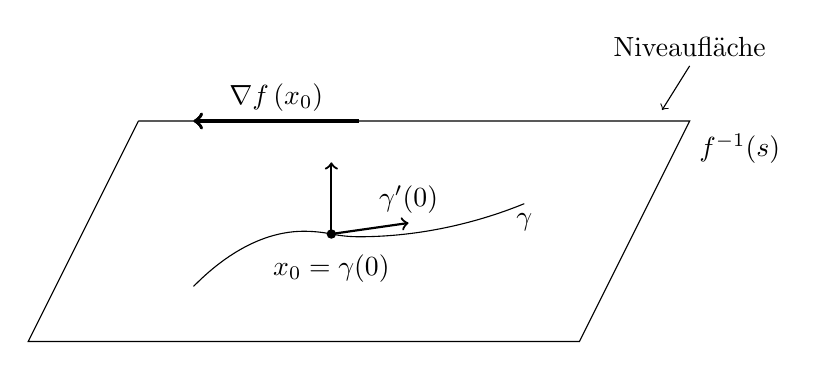
\begin{tikzpicture}[scale=0.7]
\draw[] (-5,0) -- (5,0) -- (3,-4) --(-7,-4) --  (-5,0);
\draw[<-,very thick] (-4,0) -- (-1,0);
\draw[<-,very thick] (-4,0) -- (-1,0);

\draw[] (-4,-3) parabola bend (-2,-2)(-1.5,-2.05);

\draw[] (-1.5,-2.05) parabola bend (-1,-2.1)(2,-1.5);
\draw[fill=black] (-1.5,-2.05) circle (0.075);
\draw[->,thick] (-1.5,-2.05) --(-1.5,-0.75);
\draw[->,thick] (-1.5,-2.05) --(-0.1,-1.85);
\draw (-1.5,-2.25) node[anchor=north] {$x_0=\gamma(0)$};
\draw (-0.1,-1.85) node[anchor=south] {$\gamma'(0)$};
\draw (2,-1.5) node[anchor=north] {$\gamma$};
\draw (-2.5,0) node[anchor=south] {$\nabla f\left( x_0\right)$};
\draw (5,-0.5) node[anchor=west] {$f^{-1}(s)$};
\draw [<-] (4.5,0.2) -- (5,1) node[anchor=south]{Niveaufläche};

\end{tikzpicture}
\end{center}

Dann gilt $f\left( \gamma (t)\right)=s$, $\forall t\in\lbrack -1,1\rbrack$ und es folgt aus der Kettenregel
\[\begin{array}{l}%Find if there is a better way to do this
\frac{d}{{dt}}\left( {f\left( {\gamma (t)} \right)} \right) = \frac{d}{{dt}}(s) = 0\\
\hspace{5mm} \Downarrow \\
df\left( {\gamma (t)} \right) \cdot \gamma '(t) = 0 =  < \nabla f\left( {\gamma (t)} \right),\gamma '(t) >
\end{array}\]
Insbesondere $0=df\left(\gamma (0)\right)\cdot\gamma'(0)= < \nabla f\left( x_0\right),\gamma'(0) >$ d.h. $\nabla f\left( x_0\right)$ steht senkrecht zur Niveauflache von $f$ durch $x_0$
\subsubsection*{Beispiel}
Sei $f(x,y)=\frac{x^2-y^2}{2}$, $x,y\in\R^2$ \[\nabla f(x,y)=(x,-y)\] Sei $\left( x_0,y_0\right) = (1,-1)$ \[\nabla f(1,-1)=(1,1)\hspace{10mm} \left( \nabla f(1,-1)\right) = \sqrt{2}\] \[\frac{\nabla f}{\abs{ \nabla f}}(1,-1)=\frac{1}{\sqrt{2}}(1,1)\]
\item Im Punkt $P$ biegt der Bergweg ab; nach Südosten geht er mit 25\% Steigung bergauf, nach Süden mit 20\% Gefälle bergab. Der wanderer im Nebel möchte über die Wiese möglichst rasch zum Gipfel. In welche Richtung muss er gehen und wie steil ist es dorthin?\\

Wir legen das Koordinatensystem so, dass die $x-$Achse nach Osten und die $y-$Achse nach Norden zeigt, und setzen voraus, dass die Höhenfunktion $h$ differenzierbar ist. Wir wollen ihren Gradienten in $P$ $\nabla h(P)$ bestimmen. Nach Voraussetzung hat $h$ die beiden Richtungsableitungen \[dh\left( P\right)\left( v_1\right)=0.25\hspace{10mm}dh\left( P\right)\left(  v_2\right)=-0.2\] wobei \[v_1=\left( \frac{1}{\sqrt{2}},-\frac{1}{\sqrt{2}}\right)\hspace{10mm}v_2=(0,-1)\]

\begin{center}
\begin{tikzpicture}[scale=0.7]
\draw[<->] (0,-1.5) node[anchor=north] {S} -- (0,2.5) node[anchor=south] {N} ;
\draw[<->] (-2.5,0) node [anchor = east]{W}-- (2.5,0) node[anchor = west]{E};
\draw[very thick,->] (0,0) -- (0,-1) node[anchor=east]{$v_2$};
\draw[very thick,->] (0,0) -- (0.7071067811865475244008443621048490392848359376884740,-0.7071067811865475244008443621048490392848359376884740) node[anchor=north]{$v_1$};
\end{tikzpicture}
\end{center}


\begin{align*}
dh \left( P\right) \left( v_1\right) = &\left( \frac{\partial h}{\partial x}\left(P\right), \frac{\partial h}{\partial y}\left(P\right)\right)\cdot v_1\\
= & \frac{\partial h}{\partial x}\left(P\right)\frac{1}{\sqrt{2}} +\frac{\partial h}{\partial y}\left( P\right) \left(-\frac{1}{\sqrt{2}}\right) = \frac{1}{4}\\
dh \left( P\right) \left( v_2\right) = &\left( \frac{\partial h}{\partial x}\left(P\right)\right) (0) - \frac{\partial h}{\partial y}\left(P\right)(-1)=-\frac{1}{5}
\end{align*}
Durch Lösen des linearen Gleichungssystem folgen wir:
\[\frac{\partial h}{\partial x}\left( P\right) = \frac{\sqrt{2}}{4}+\frac{1}{5}, \frac{\partial h}{\partial y}\left( P\right) = \frac{1}{5}\]
Die Richtung des Gradients ist somit \[ \arg\nabla h\left( P \right) = \arctan{\frac{\frac{1}{5}}{\frac{\sqrt{2}}{4}+ \frac{1}{5}}}\cong 19.86\text{\textdegree} \]
und die Steigung in diese Richtung ist
\[\abs{ \nabla h\left( P\right) } = \sqrt{\left( \frac{\sqrt{2}}{4}+\frac{1}{5}\right)^2 + \left( \frac{1}{5}\right)^2} \cong 0.59 = 59\%\] 
\end{enumerate}

\section{Wegintegrale}
Wir haben in Bemerkung 8.29 gesehen, dass man mittels dem üblichen Skalarprodukt $<,>$ von $1-$Formen zu Vektorfeldern und umgekehrt übergehen kann. \\

In diesem Kapitel werden wir das ``Wegintegral'' von $1-$Formen oder \todo{can't read, page 162 middle} von Vektorfeldern längs eine Kurve studieren. Dazu untersuchen wir zunächst Kurven in $\R^n$

\subsection*{Parameterdarstellung einer Kurve}
Sei $\gamma\subset\R^n$ eine Kurve. Eine Parameterdarstellung (PD) von $\gamma$ ist eine Funktion
\begin{align*}
\gamma : I=\lbrack a,b\rbrack &\to\R^n\\
t &\to \gamma (t)
\end{align*}
wobei $\gamma\left( t\right)$ ein Punkt $\gamma$ ist und jeder Punkt auf $\gamma$ kann als $\gamma\left( t\right)$ dargestellt werden
\[\gamma\left( t\right) = \left( \gamma_1 (t),\dots,\gamma_n (t)\right)\]
Die positive Richtung von $\gamma$ ist die Richtung mit der die Kurve durchgelaufen wird
\subsubsection*{Beispiel 8.32}
\begin{enumerate}
\item \[\gamma (t)=\left( a_1 +b_1 t,a_2 +b_2 t,a_3 +b_3 t\right)\text{, }t\in\R\]
ist die Parameterdarstellung einer Gerade durch den Punkt $a=\left( a_1,a_2,a_3\right)$ und parallel zum Vektor $\left( b_1,b_2,b_3\right)$

\begin{center}
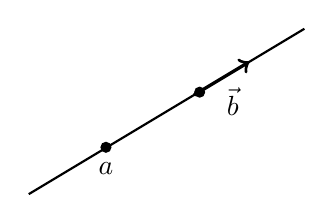
\begin{tikzpicture}[scale=0.7]
\draw[thick] (0,0) -- (5,3) ;

\node[circle,fill=black,inner sep=0.5mm] (a) at (1.4,0.85) {};
\draw (1.4,0.75) node[anchor=north] {$a$};
\draw[very thick,->] (3,1.8) -- (4,2.4) ;

\node[circle,fill=black,inner sep=0.5mm] (a) at (3.1,1.85) {};
\draw (3.7,2.1) node[anchor=north] {$\vec b$};

\end{tikzpicture}
\end{center}

\item $\gamma (t)=\left( a\cos t,b\sin t\right)$ ist eine Parameterdarstellung einer Ellipse
\begin{figure}[H]
\begin{minipage}[b]{0.45\linewidth}

%LEFT
\[\frac{x^2}{a^2}+\frac{y^2}{b^2}=1\]
\[t\in\lbrack 0,2\pi\rbrack\]
\end{minipage}
\hspace{0.5cm}
\begin{minipage}[b]{0.45\linewidth}

%RIGHT
\begin{center}
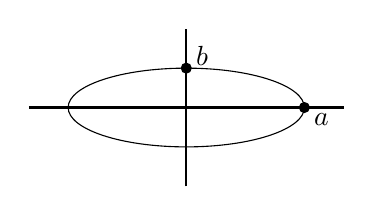
\begin{tikzpicture}[scale=0.5]
\draw[thick] (0,-2) -- (0,2) ;
\draw[thick] (-4,0) -- (4,0) ;

\node[circle,fill=black,inner sep=0.5mm] (a) at (3,0) {} ;
\node[circle,fill=black,inner sep=0.5mm] (a) at (0,1) {};
\draw (0,0) ellipse (3 and 1);

\draw (3,-0.3) node[anchor=west]{$a$};
\draw (0,1.3) node[anchor=west]{$b$};
\end{tikzpicture}
\end{center}

\end{minipage}
\end{figure}
\item $\gamma_1 (t)=\left( a\cos t,b\sin t, ct\right)$, $t\in\lbrack 0,2\pi\rbrack$ ist eine Parameterdarstellung einer elliptischen Helix
\begin{center}
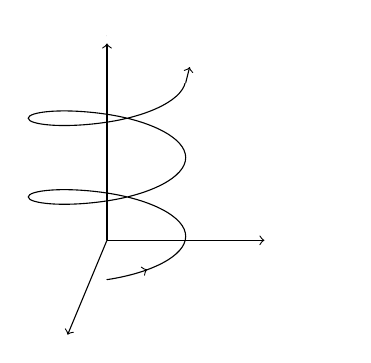
\begin{tikzpicture}
%DON'T CHANGE THE ORDER OF THE TWO FOLLOWING COMMANDS!!
\draw[decoration={aspect=0.3, segment length=10mm, amplitude=10mm,coil},decorate] (0,3.1) -- (0,0);
\fill [white] (3,3.2) rectangle (0,2.5);
\draw[->] (1,2.5) -- (1.05,2.7);
\draw[->] (0.5,0.125) -- (0.51,0.129);
\draw[->] (0,0.5) -- (0,3);
\draw[->] (0,0.5) -- (2,0.5);
\draw[->] (0,0.5) -- (-0.5,-0.7);
\end{tikzpicture}
\end{center}
$\gamma_2 (t)=\left( a\cos t,-b\sin t, c(2\pi -t)\right)$, $t\in\lbrack 0,2\pi\rbrack$ ist die Parameterdarstellung der gleichen Kurve wobei die Richtung umgekehrt ist

\begin{center}
\begin{tikzpicture}[scale=1]

\draw[bend left](0,0) to (6,2);
\draw[fill=black] (1.5,1.3) circle (0.05);
\draw[fill=black] (3,1.97) circle (0.05);
\draw[->](1.5,1.3) to (2.5,2);
\draw[](1.5,1.3) to (0.3,-2);
\draw[](3,1.97) to (0.85,-0.5);
\draw[](2.2,1) node [anchor=west]{$\gamma(t+h)$};
\draw[](1.2,0.3) node [anchor=east]{$\gamma(t)$};
\draw[](6,2) node [anchor=west]{$\gamma(t)$};
\end{tikzpicture}
\end{center}

Der Tangentialvektor zur Kurve an der Stelle $\gamma (t)$ ist $\gamma' (t)$ \[\gamma'(t)=\left( \gamma_1'(t),\gamma_2'(t),\dots, \gamma_n'(t)\right)\]
\todo{Do I have to include the example?? page 164 bottom}
\end{enumerate}

\begin{definition}{8.33}
Das Wegintegral von $\vartheta$ längs $\gamma$
\[\int\limits_\gamma  {vd\vec s}  = \int\limits_\gamma  {v(\gamma )d\gamma : = \int\limits_a^b { < v\left( {\gamma \left( t \right)} \right),\gamma '(t) > dt} } \] ${vd\vec s}=\gamma'(t)dt$ heisst gerichtetes Längenelement
\end{definition}
\subsubsection*{Beispiel 8.34}
Ein einführendes Beispiel: Sei $m$ ein Massenpunkt, der sich unter den Einfluss eines Kraftfeldes $F:\R^2\to\R$ bewegt.\\

Der Massenpunkt wird durch eine konstante Kraft $\overrightarrow F $ längs einer Geraden um den Vektor $\vec s$ verschoben. \\

Die dabei verrichtete Arbeit ist definitionsgemäss das Skalarprodukt aus dem Kraftvektor $\overrightarrow F $ und dem Verschiebungsvektor $\vec s$.

\begin{center}
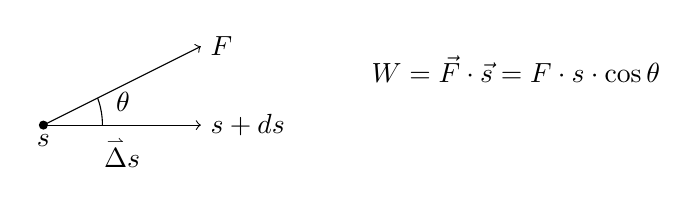
\begin{tikzpicture}
\draw[->] (0,0) -- (2,0);
\draw[->] (0,0) -- (2,1);
\draw[fill=black] (0,0) circle (0.05);

\draw(0.8,0.3) node [anchor=west]{$\theta$};
\draw (0.75,0) arc (0:20:1cm);
\draw(2,1) node [anchor=west]{$F$};
\draw(0,0) node [anchor=north]{$s$};
\draw(2,0) node [anchor=west]{$s+ds$};
\draw(1,0) node [anchor=north]{$\mathord{\buildrel{\lower3pt\hbox{$\scriptscriptstyle\rightharpoonup$}}
\over \Delta } s$};
\draw(6,1) node [anchor=north]{$W=\vec F\cdot \vec s=F\cdot s\cdot\cos\theta$};
\end{tikzpicture}
\end{center}

\noindent\underline{Allgemeiner Fall}\\
Verschiebung längs einer Kurve $\gamma$ in einem Kraftfeld $F=\left( P(x,y),Q(x,y)\right)$
\begin{center}
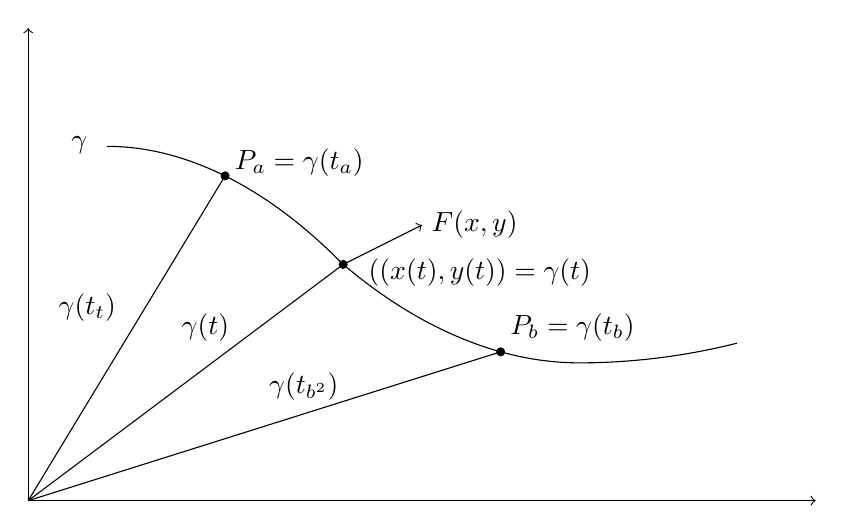
\begin{tikzpicture}
\draw[->] (0,0) -- (10,0);
\draw[->] (0,0) -- (0,6);

\draw (1,4.5) parabola bend (1,4.5)(4,3);
\draw (4,3) parabola bend (7,1.75)(9,2);

\draw[] (0,0) -- (2.5,4.125);
\draw[fill=black] (2.5,4.125) circle (0.05);
\draw(2.5,4.3) node [anchor=west]{$P_a=\gamma(t_a)$};

\draw[] (0,0) -- (4,3);
\draw[fill=black] (4,3) circle (0.05);
\draw(4.2,2.9) node [anchor=west]{$\left( (x(t),y(t)\right)=\gamma(t)$};
\draw[->] (4,3) -- (5,3.5);
\draw(5,3.5) node [anchor=west]{$F(x,y)$};


\draw[] (0,0) -- (6,1.89);
\draw[fill=black] (6,1.89) circle (0.05);
\draw(6,2.2) node [anchor=west]{$P_b=\gamma(t_b)$};

\draw(0.65,4.75) node [anchor=north]{$\gamma$};

\draw(0.75,2.75) node [anchor=north]{$\gamma(t_t)$};
\draw(2.25,2.5) node [anchor=north]{$\gamma(t)$};
\draw(3.5,1.75) node [anchor=north]{$\gamma(t_{b^2})$};

\end{tikzpicture}
\end{center}

$\Delta W= F\cdot \Delta (\gamma)=$ Kraftkomponente entlang des Weges mal zurückgelegter Weg. \\

Da sich Betrag und Richtung der Kraft sowie der jeweilige Winkel zum Weg vom Punkt zu Punkt ändern, gilt das zur Berechnung notwendige Skalarprodukt näherungsweise jeweils nur für ein Wegelement $\overrightarrow\Delta r$. Die Berechnung der Arbeit erfolgt daher in folgender Weise:
\begin{enumerate}[\indent a)]
\item Zerlegung des Weges in Teilabschnitte \[\Delta \gamma_1=\gamma (t_{i+1})-\gamma(t_i)=\frac{\Delta \gamma}{\Delta t}\cdot \Delta t\]
\item Ermittlung der Arbeit \todo{can't read, page 167 middle; limenet: plus, grammar is totally wrong} Kraft: \[F\left( {\gamma \left( {{t_i}} \right)} \right) = F\left( {x\left( {{t_i}} \right),y\left( {{t_i}} \right)} \right)\]
\item Berechnen der Arbeit je Teilabschnitt-Skalarprodukt \[\Delta {W_i} = F\left( {x\left( {{t_i}} \right),y\left( {{t_i}} \right)} \right) \cdot \Delta {\gamma _i}\]
\item Aufsummieren der Teil-Arbeit \[W \approx \sum {\Delta {W_i} = \sum {F\left( {x\left( {{t_i}} \right),y\left( {{t_i}} \right)} \right)} }  \cdot \underbrace {\Delta \gamma }_{\frac{{\Delta \gamma }}{{\Delta t}} \cdot \Delta t}\]
\item Durch Verkleinerung des Wegelementes enthält man den exakten Wert der geleisteten Arbeit
\begin{align*}
W = &\int\limits_a^b {F\left( {\gamma \left( t \right)} \right)}  \cdot \gamma '\left( t \right)dt\\
 = &\int\limits_a^b { < F\left( {\gamma \left( t \right)} \right)} ,\gamma '\left( t \right) > dt
\end{align*}
\end{enumerate}
\subsubsection*{Bemerkung 8.35}
Wir können das Wegintegral auch mit Differentialformen formulieren. Sei
\begin{align*}
v:\Omega &\to\R^n\\
x &\to\left( v^i(x)\right)_{i=1}^n
\end{align*}
ein stetiges Vektorfeld ($v^i(x):\R^n\to\R$ stetig) dann ist durch $\lambda (x)(\omega):=< v(x),\omega >$ eine $1-$Form $\lambda (x)\in L\left( \R^n,\R\right)$ definiert
\begin{align*}
\int\limits_\gamma  {vd\vec s}  = &\int\limits_a^b { < v\left( {\gamma (t)} \right),\gamma '(t) > dt}\\
 = &\int\limits_a^b {\lambda \left( {\gamma \left( t \right)} \right)\left( {\gamma '\left( t \right)} \right)dt}
\end{align*}

\noindent\underline{Umgekehrt}\\

\noindent Sei $\lambda :\Omega\to L\left( \R^n,\R\right)$ eine $1-$Form die im folgenden Sinn stetig ist: \\

Sei
\begin{align*}
\gamma :\lbrack a,b\rbrack &\to\Omega\\
t &\to\left( \gamma^1 (t), \gamma^2 (t),\dots ,\gamma^n (t) \right)
\end{align*}
ein $C^1-$Weg. Dann ist
\begin{align*}
\lbrack a,b\rbrack \to &\R\\
t\to &\lambda\left( \gamma (t)\right)\left( \gamma' (t)\right)\\
& = \sum{\lambda_i\left(\gamma(t)\right)\cdot\frac{d\gamma^i}{dt}(t)}
\end{align*}
eine stetige Funktion. Somit ist das Integral $\int\limits_a^b {\lambda \left( {\gamma \left( t \right)} \right)\left( {\gamma '\left( t \right)} \right)dt} $ wohl definiert.

\begin{definition}{8.36}
Das Wegintegral von $\gamma\in L\left( \R^n,\R\right)$ längs $\gamma$ ist \[\int\limits_\gamma  \lambda  : = \int\limits_a^b {\lambda \left( {\gamma (t)} \right)\left( {\gamma '(t)} \right)dt} \]
\end{definition}

\subsubsection*{Beispiel 8.37}
\begin{enumerate}
\item Sei $\gamma\in C^1\left(\lbrack 0,2\pi\rbrack =\R^2\right)$ mit
\[\begin{array}{*{20}{c}}
{\gamma (t) = \left( {\begin{array}{*{20}{c}}
{\cos t}\\
{\sin t}
\end{array}} \right)}&{}\\
{}&{0 \le t \le 2\pi }\\
{\gamma '(t) = \left( {\begin{array}{*{20}{c}}
{ - \sin t}\\
{\cos t}
\end{array}} \right)}&{}
\end{array}\]
eine Parametrisierung des Einheitskreises $\lambda = \lambda (x,y)$ die $1-$Form mit \[\lambda (x,y)=-ydx+xdy\hspace{10mm}(x,y)\in\R^2\]
Dann gilt
\begin{align*}
\int\limits_\gamma  \lambda   = &\int\limits_0^{2\pi } {\underbrace {\left( { - \sin t,\cos t} \right)}_{\lambda (\gamma (t))} \cdot \underbrace {\left( {\begin{array}{*{20}{c}}
{ - \sin t}\\
{\cos t}
\end{array}} \right)}_{\gamma '(t)}dt} \\
= &\int\limits_0^{2\pi } {\left( {{{\sin }^2}t + {{\cos }^2}t} \right)dt}  = 2\pi
\end{align*}
\item Sei $\gamma (x,y)=3x^2ydx + \left( x^3+1\right)dy$. Wir betrachten das Kurvenintegral längs verschiedener Wege
\begin{multicols}{2}
\begin{align*}
\gamma_1(t)&=(t,t), 0\leq t\leq 1\\
\gamma_1'(t)&=(1,1)\\
\gamma_2(t)&=(t,t^2), 0\leq t\leq 1\\
\gamma_2'(t)&=(1,2t)\\
\end{align*}
\null\vfill
\columnbreak
\begin{center}
\begin{tikzpicture}[scale=0.6]
		\node [] (0) at (0, 0) {};
		\node [] (1) at (4, 4) {};
\begin{scope}[decoration={
    markings,
    mark=at position 0.5 with {\arrow{>}}}
    ] 
		\draw [postaction={decorate},bend right] (0.center) to (1.center);
		\draw [postaction={decorate}] (0.center) to (1.center);
		\end{scope}
\draw[->](-0.5,0) --(5,0);
\draw[->](0,-0.5) --(0,5);
\draw(-0.2,0) node [anchor=north]{0};	
\draw[fill=black] (0,0) circle (0.05);	
\draw[fill=black] (4,4) circle (0.05);	
\draw(2,2.1) node [anchor=south]{$\gamma_1$};
\draw(3.2,1.05) node [anchor=south]{$\gamma_2$};
\draw(4,4) node [anchor=west]{$(1,1)$};
\end{tikzpicture}
\end{center}
\null\vfill
\end{multicols}
\vspace{-15mm}
\begin{align*}
&\int\limits_{{\gamma _1}} \lambda   = \int {3{x^2}ydx + \left( {{x^3} + 1} \right)dy}  = \int\limits_0^1 {\left( {3{t^3} + \left( {{t^3} + 1} \right)} \right)dt = 2}\\
&\int\limits_\gamma  \lambda   = \int\limits_0^1 {\left( {3{t^4} + \left( {{t^3} + 1} \right) \cdot 2t} \right)dt = 2}
\end{align*}
\subsubsection*{Bemerkung}\todo{is  this inside the enumerated list or out?? page 170 bottom}
Sei $f(x,y)=x^3y+y$. Dann ist  \[df(x+y)=3x^2ydx+\left( x^3+1\right) dy\] und \[f(1,1)-f(0,0)=(1+1)-(0,0)=2\]
Wir können den Begriff des Wegintegrals auf Wege erweitern, die stückweise $C^1$ sind. Ein stückweiser $C^1-$Weg ist eine stetige Abbildung $\gamma :\lbrack a,b\rbrack\to\R^n$ mit einer Unterteilung des Intervalls
\[a=a_0 < a_1 < a_2 < \dots <a_n = b\]
so dass \[{\left. \gamma  \right|_{\left[ {{a_i},{a_{i + 1}}} \right]}} = \left[ {{a_i},{a_{i + 1}}} \right] \to \R^n \] $C^1$ ist.\\

\noindent d.h. $t\to\gamma'(t)$ ist auf $\left( a_i, a_{i+1}\right)$ stetig und erweitert sich stetig auf $\lbrack a_i, a_{i+1}\rbrack$
\subsubsection*{Beispiel}\todo{is  this inside the enumerated list or out?? page 171 middle}

\begin{multicols}{2}
\begin{center}
\begin{tikzpicture}[scale=0.5]
\node [] (0) at (0, 0) {};
\node[](1) at (4,0){};
\node [] (2) at (8, 2) {};
\draw [bend left=60] (0.center) to (1.center);
\draw [] (1.center) to (2.center);
\draw[fill=black] (0.center) circle (0.075);
\draw[fill=black] (1.center) circle (0.075);
\draw[fill=black] (2.center) circle (0.075);
\end{tikzpicture}
\end{center}
\columnbreak
\null\vfill
Bild eines stückweise $C^1-$Weges
\end{multicols}

Dann definiert man
\[\int\limits_\gamma  \lambda  : = \sum\limits_{t = 0}^{n - 1} {\int\limits_{{{\left. \gamma  \right|}_{\left[ {{a_i},{a_{i + 1}}} \right]}}} \lambda  } \]
Jetzt werden wir die einzige grundlegende Eigenschaften des Wegintegrals herleiten.
\end{enumerate}

\subsubsection*{Satz 8.38 (Eigenschaften des Wegintegrals)}
\begin{enumerate}[\indent E1)]
\item Das Wegintegral $\int\limits_\gamma  \lambda  $ ist unabhängig von einer orientierungserhaltenden Umparametrisierung. \\
D.h. Sei $\gamma :\lbrack a,b\rbrack\to\Omega$, $C^1$ und $\varphi :\lbrack a',b'\rbrack\to\lbrack a,b\rbrack$, $C^1$ mit $\varphi\left( a'\right)=a$, $\varphi\left( b'\right)=b$, $\varphi'\left( t\right) >0$ $\forall t\in\lbrack a', b'\rbrack$. Dann ist
\begin{align*}
\int\limits_{\gamma  \circ \varphi } \lambda   = &\int\limits_{a'}^{b'} {\lambda \left( {\gamma \left( {\varphi (t)} \right)} \right)\left( {\gamma  \circ \varphi } \right)'(t)dt} \\
 = &\int\limits_{a'}^{b'} {\lambda \left( {\gamma \left( {\varphi (t)} \right)} \right)\gamma '\left( {\varphi (t)} \right)\varphi '(t)dt} \\
 = &\int\limits_a^b {\lambda \left( {\gamma \left( s \right)} \right)\gamma '\left( s \right)ds = \int\limits_\gamma  \lambda  }
\end{align*}
Geometrisch heisst dies, dass $\int\limits_\gamma  \lambda$ nur vom Bild $\gamma\left( \lbrack a,b\rbrack\right)$ mit vorgegebenen Durchlaufsinn abhängt.
\item Seien $\gamma_1:\lbrack a_1,b_1\rbrack\to\Omega$ und $\gamma_2:\lbrack a_2,b_2\rbrack\to\Omega$ zwei Wege mit $\gamma_1\left( b_1\right)=\gamma_2\left(a_2\right)$
\begin{center}
\begin{tikzpicture}

\draw[fill=black] (4,1) circle (0.05);
\draw[fill=black] (8,0) circle (0.05);
\draw[fill=black] (0,0) circle (0.05);
\begin{scope}[decoration={
    markings,
    mark=at position 0.5 with {\arrow{>}}}
    ] 
		\draw[postaction={decorate}] (0,0) parabola bend (3,0.9)(4,1);
\draw[postaction={decorate}]  (4,1) parabola bend (5,0.9) (8,0);
		\end{scope}

\draw (4,1) node [anchor=south] {$\gamma_1(b_1)=\gamma_2(a_2)$};
\draw (2,0.85) node [anchor=south] {$\gamma_1$}; 
\draw (6,0.85) node [anchor=south] {$\gamma_2$}; 
\draw (0,0) node [anchor=north] {$\gamma_1(a_1)$};
\draw (8,0) node [anchor=north] {$\gamma_2(b_2)$}; 
\end{tikzpicture}
\end{center}
Wir definieren $\gamma_1+\gamma_2$ als Weg, der durch aneinanderhängen von $\gamma_1$ und $\gamma_2$ entsteht, d.h.
\[{\gamma _1} + {\gamma _2} = \left\{ {\begin{array}{*{20}{c}}
{{\gamma _1}(t)}&{t \in \left[ {{a_1},{b_1}} \right]}\\
{{\gamma _2}\left( {t - {b_1} + {a_2}} \right)}&{t \in \left[ {{b_1},{b_1} + {b_2} - {a_2}} \right]}
\end{array}} \right.\]
Dann gilt \[\int\limits_{{\gamma _1} + {\gamma _2}} \lambda   = \int\limits_{{\gamma _1}} \lambda   + \int\limits_{{\gamma _2}} \lambda  \]
\item Sei $\gamma:\lbrack a,b\rbrack\to\Omega$ ein Weg. Dann sei $-\gamma:\lbrack a,b\rbrack\to\Omega$ der gleiche Weg aber im entgegengesetzten Durchlaufsinn, d.h. $\left( -\gamma\right) (t)=\gamma\left( -t+a+b\right)$

\begin{center}
\begin{tikzpicture}[scale=0.75]

\begin{scope}[decoration={
    markings,
    mark=at position 0.5 with {\arrow{>}}}
    ] 
		\draw[postaction={decorate}]  (0,0) parabola bend (2,1.5)(2,1.5);
\draw[postaction={decorate}](2,1.5) parabola bend (2,1.5)(4,3);
		\end{scope}
		
\begin{scope}[decoration={
    markings,
    mark=at position 0.5 with {\arrow{<}}}
    ] 
		\draw[postaction={decorate}]  (3,0) parabola bend (5,1.5)(5,1.5);
\draw[postaction={decorate}](5,1.5) parabola bend (5,1.5)(7,3);
		\end{scope}

\draw (2,2.2) node [anchor=north]{$\gamma$};
\draw (5,0.8) node [anchor=south]{$-\gamma$};

\end{tikzpicture}
\end{center}

Dann gilt \[\int\limits_{ - \gamma } \lambda   =  - \int\limits_\gamma  \lambda  \]
\item Sei $f:\Omega\to\R$ eine $C^1-$Funktion, sowie $\gamma:\lbrack a,b\rbrack\to\Omega$ stückweise $C^1$. Dann gilt \[\int\limits_\gamma  {df}  = f\left( {\gamma \left( b \right)} \right) - f\left( {\gamma \left( a \right)} \right)\]
$\gamma$ ist $C^1$, dann ist
\begin{align*}
\int\limits_\gamma  {df}  = & \int\limits_a^b {df\left( {\gamma \left( t \right)} \right)\gamma '\left( t \right)dt} \\
\mathop  = & \int\limits_a^b {\frac{d}{{dt}}\left( {f \circ \gamma } \right)\left( t \right)dt}\\
 = &\left( {f \circ \gamma } \right)\left( b \right) - \left( {f \circ \gamma } \right)\left( a \right)\\
 = & f\left( {\gamma \left( b \right)} \right) - f\left( {\gamma \left( a \right)} \right)
\end{align*}
Mittels des Wegintegrals können wir die $C^1-$Funktionen charakterisieren, deren Differentiale verschwinden.
\end{enumerate}

\subsubsection*{Satz 8.39}
Sei $\Omega$ ``offen'' und $C^1-$wegzusammenhängend. Sei $f\in C^1\left(\Omega\right)$. Falls $df(x)=0$, $\forall x\in\Omega$, so ist $f$ konstant.
\subsubsection*{Beweis}
Wenn $\Omega$ wegzusammenhängend ist, heisst das, dass zu je zwei Punkten $x,y\in\Omega$ gibt es in $C^1-$Weg $\gamma :\lbrack 0,1\rbrack\to\gamma$ mit $\gamma(0)=x$ und $\gamma(1)=y$, $\gamma\left(\lbrack 0,1\rbrack\right)\subset\Omega$. Dann folgt
\begin{align*}
f(y)-f(x)&= f\left(\gamma(1)\right)-f\left(\gamma(0)\right)\\
= &\int\limits_{\gamma} df = 0
\end{align*}
$\Rightarrow f(y)=f(x)$, $\forall x,y\in\Omega\Rightarrow f$ ist konstant.\\

\noindent\underline{Frage:} Wann ist eine $1-$Form $\lambda$, von der Form $\lambda = df$, d.h. das Differential einer Funktion? D.h. gegeben eine $1-$Form $\lambda$, gibt es eine Funktion $f:\Omega\to\R$ s.d. $df=\lambda$\\?

Wenn es ein $f:\Omega\to\R$ gibt, so dass $df=\lambda$, heisst $f$ ein Potential. (Potential ist wie eine Stammfunktion für eine $1-$Form). Mittels Wegintegral stellen wir jetzt ein Kriterium auf.

\subsubsection*{Satz 8.30}
Sei $\lambda\in\Omega\to L\left( \R^n,\R\right)$ eine stetige $1-$Form. Folgende Aussagen sind äquivalent
\begin{enumerate}
\item Es gibt $f\in C^1\left( \Omega\right)$ mit $df=\Omega$
\item Für je zwei stückweise $C^1-$Wege $\gamma_i=\lbrack a_i,b_i\rbrack\to\Omega$ mit den selben Anfangs- und Endpunkten (d.h. $\gamma_1\left( a_1\right)=\gamma_2\left(a_2\right)$, $\gamma_1\left( b_1\right)=\gamma_2\left(b_2\right)$), gilt \[\int\limits_{{\gamma _1}} \lambda   = \int\limits_{{\gamma _2}} \lambda  \]
\item Für jeden geschlossenen $C^1$Weg $\gamma$ gilt \[\int\limits_\gamma  \lambda   = 0\]
\end{enumerate}

\subsubsection*{Beweis}
\begin{enumerate}[align=left]
\item[$(1)\Rightarrow (2)$:] Folgt aus E4)
\item[$(2)\Leftrightarrow (3)$:] Klar
\item[$(2)\Rightarrow (1)$:] Sei $p_0\in\Omega$; für jedes $x\in\Omega$. Sei $\gamma:\lbrack 0,1\rbrack\to\Omega$ stückweise $C^1$ mit $\gamma(0)=p_0$, $\gamma(1)=x$. Definiere $f(x): = \int\limits_\gamma  \lambda $.\\

Dann ist $f$ nach Annahme (2) wohl definiert (d.h. unabhängig vom Weg von $p_0$ nach $x$) (Wir können $f$ auch mit $\int\limits_{{p_0}}^x \lambda  $ bezeichnen)
\end{enumerate}

\subsubsection*{Behauptung}
$f\in C^1\left( \Omega\right)$ und $df=\lambda$. Um zu zeigen, dass $df=\lambda$ müssen wir zeigen, dass für $x,x_0\in\Omega$
\[f\left(x\right)-f\left(x_0\right)=\lambda\left(x_0\right)\left( x-x_0\right)+R\left( x,x_0\right)\] mit $\frac{R\left( x,x_0\right)}{\abs{ x-x_0}}\to 0$.\\

\noindent Sei $x_0\in\R$. Sei $\gamma_1:\lbrack -1,0\rbrack\to\Omega$ ein Weg von $p_0$ nach $x_0$. Dann gilt \[\int\limits_{{\gamma _1}} \lambda   = f\left( {{x_0}} \right)\]
Sei
\begin{align*}
\gamma_x:\lbrack 0,1\rbrack &\to\Omega\\
t &\to (1-t)x_0+tx
\end{align*}

\begin{center}
\begin{tikzpicture}[scale=0.5]


		\node [] (0) at (-0.25, 0) {};
		\node [] (1) at (-2, 3) {};
		\node [] (2) at (-4, 0) {};
		\draw [] (1.center) to (0.center);
		
		\begin{scope}[decoration={
    markings,
    mark=at position 0.5 with {\arrow{>}}}
    ] 
		\draw [postaction={decorate},bend left=15] (2.center) to (1.center);
		\end{scope}
		\begin{scope}[decoration={
    markings,
    mark=at position 0.5 with {\arrow{>}}}
    ] 
		\draw [postaction={decorate},bend right=15] (2.center) to (0.center);	
		\end{scope}		
		


		\draw[] (-0.25,0) circle (4.5);
\draw[->](-0.25,0)--(3.5,2.5);
\draw[fill=black] (0.center) circle (0.075);
\draw[fill=black] (1.center) circle (0.075);
\draw[fill=black] (2.center) circle (0.075);
\draw (1.5,1.5) node [anchor=south]{$r$};
\draw (1.north) node [anchor=south]{$x$};
\draw (0.south) node [anchor=north]{$x_0$};
\draw (2.south) node [anchor=north]{$p_0$};
\draw (-2,-0.5) node [anchor=north]{$\gamma_1$};
\draw (-0.65,2) node [anchor=north]{$\gamma_x$};
\draw (-3.75,2) node [anchor=north]{$\gamma$};
\end{tikzpicture}
\end{center}

Um $\gamma^x\left( \lbrack 0,1\rbrack\right)\subset\Omega$ zu garantieren, nehmen wir $r>0$, so dass $B_r\left( x_0\right)\subset\Omega$ und nehmen an, dass $x\in B_r\left( x_0\right)$. Dann ist
\[f(x) = \int\limits_{{\gamma _1} + {\gamma _x}} \lambda   = \int\limits_{{\gamma _1}} \lambda   + \int\limits_{{\gamma _x}} \lambda   = f\left( {{x_0}} \right) + \int\limits_{{\gamma ^x}} \lambda  \]
Nun ist
\begin{align*}
\int\limits_{{\gamma ^x}} \lambda   = &\int\limits_0^1 {\lambda \left( {{\gamma _x}\left( t \right)} \right){\gamma _x}'\left( t \right)} dt\\
 = &\int\limits_0^1 {\lambda \left( {{\gamma _x}\left( t \right)} \right)\left( {x - {x_0}} \right)} dt\\
 = &\lambda \left( {{x_0}} \right)\left( {x - {x_0}} \right) + \int\limits_0^1 {\left( {\lambda \left( {{\gamma ^x}\left( t \right)} \right) - \lambda \left( {{x_0}} \right)} \right)\left( {x - {x_0}} \right)dt}
\end{align*}

Sei $\lambda  = \sum {{\lambda ^i}d{x^i}} $ dann ist obiges Integral gleich
\begin{align*}
&\sum {\int\limits_0^1 {\left[ {{\lambda _i}\left( {{\gamma ^x}\left( t \right)} \right) - {\lambda _i}\left( {{x_0}} \right)} \right]\left( {{x^i} - x_0^i} \right)dt} }\\
 \le &\sum {{{\left( {\int\limits_0^1 {{{\left[ {{\lambda _i}\left( {{\gamma ^x}\left( t \right)} \right) - {\lambda _i}\left( {{x_0}} \right)} \right]}^2}} } \right)}^{\frac{1}{2}}}} \abs{ {x - {x_0}} }
\end{align*}
Also $f\left( x \right) - f\left( {{x_0}} \right) = \lambda \left( {{x_0}} \right)\left( {x - {x_0}} \right) + R\left( {x,{x_0}} \right)$, wobei
\[\frac{{R\left( {x - {x_0}} \right)}}{{\abs{ {x - {x_0}} }}} \le {\left( {\sum\limits_{i = 1}^n {{{\left( {\int\limits_0^1 {\left( {{\lambda _i}\left( {{\gamma ^x}\left( t \right)} \right) - {\lambda _i}\left( {{x_0}} \right)} \right)dt} } \right)}^2}} } \right)^{\frac{1}{2}}}\]
Aus der Stetigkeit der \todo{Can't read, page 179 bottom} folgt, dass
\[\mathop {\lim }\limits_{x \to {x_0}} \frac{{R\left( {x,{x_0}} \right)}}{{\abs{ {x - {x_0}} }}} \to 0\]

\subsubsection*{Beispiel 8.31}
\begin{enumerate}
\item Sei $\lambda = 2xy^2dx+2x^2ydy$. \\

\noindent\underline{Ansatz:} \[f\left(x,y\right)=\int\limits_{\gamma_{\left( x,y\right)}}\lambda\]
wobei $\gamma_{\left( x,y\right)}\left(t\right)=\left(t_x,t_y\right)$, $t\in\left( 0,1\right)$. Dann ist

\begin{align*}
\int\limits_\gamma  \lambda   = &\int\limits_0^1 {\lambda \left( {tx,ty} \right)\left( {x,y} \right)dt} \\
= &\int\limits_0^1 {\left[ {2\left( {tx} \right){{\left( {ty} \right)}^2} \cdot x + 2{{\left( {tx} \right)}^2}\left( {ty} \right) \cdot y} \right]dt} \\
= & 4{x^2}{y^2}\int\limits_0^1 {{t^3}} dt = {x^2}{y^2}
\end{align*}
und $df\left( x,y\right)=2xy^2dx+2x^2ydy$.\\

\noindent\underline{Oder:} Ansatz:
\[df:\lambda \Rightarrow\frac{\partial f}{\partial x}=  2xy^2, \frac{\partial f}{\partial y}=  2x^2y\]
\[\Rightarrow \frac{\partial f}{\partial x}=2xy^2 \Rightarrow f\left( x,y \right) = \int 2xy^2 dx =  x^2y^2+C\left( y\right)\]
\[\Rightarrow\frac{\partial f}{\partial y}=2x^2y+\frac{d}{dy}C\left(y\right)=2x^2y \Rightarrow \frac{d}{dy}C\left( y\right) =  0 \Rightarrow C\left( y\right) = \text{ Konstant}\]
\[\Rightarrow f\left( x,y\right)=  x^2y^2+C\]
\end{enumerate}\todo{Where is number 2?? page 180}
Analog wie für $1-$Formen kann man Satz 8.30 für Vektorfelder formulieren

\begin{definition}{8.32}
Ein Vektorfeld $v:\Omega\to\R^n$ heisst konservativ, falls $\forall\gamma:\lbrack 0,1\rbrack\to\Omega$ geschlossen ist \[\int\limits_\gamma v ds=0\]
\end{definition}
Aus Satz 8.30 folgt
\subsubsection*{Satz 8.33}
Für ein stetiges Vektorfeld $v:\Omega\to\R^n$ sind folgende Aussagen äquivalent
\begin{enumerate}
\item $v$ ist konservativ
\item Es gibt $f\in C^1\left( \Omega\right)$ mit $v=\nabla f$. In diesem Fall heisst $v$ Potentialfeld mit dem Potential $f$.
\end{enumerate}

Im nächsten Kapitel, mittels höheren partiellen Ableitungen, erhalten wir eine einfache zu \todo{can't understand, page 182 top} notwendige Bedingung für ein konservatives Vektorfeld. Wir werden sehen, dass
\[v = {\left( {{v^i}} \right)_{1 \le i \le n}} \in C^1\left( {\Omega ,\R^n} \right)\text{ konservative }\]
\[\Rightarrow \frac{\partial v^i}{\partial x^j}=\frac{\partial v^j}{\partial x^i}\hspace{5mm}1\leq i,j\leq n\]

\section{Höhere Ableitungen}
\begin{definition}{8.44}
$f:\Omega\to\R$, $\Omega\subset\R^n$ $f\in C^1\left( \Omega\right)$ heisst von Klasse $C^2$ falls $\frac{\partial f}{\partial x^i}\in C^1{\left( \Omega\right)}_{1\leq i\leq n}$
\end{definition}\todo{Where does the definition end? page 183 top}
Für ein beliebiges $m$, heisst die Funktion $f\in C^1\left( \omega\right)$ heisst von der Klasse $C^m$, $f\in C^m\left( \omega\right)$, falls $\frac{\partial f}{\partial x^i}\in C^{m-1}\left( \Omega\right)$, $1\leq i\leq n$\\

Für ein $f\in C^2\left( \Omega\right)$, heissen die Funktionen \[\frac{{{\partial ^2}f}}{{\partial {x^i}\partial {x^j}}}: = \frac{\partial }{{\partial {x^i}}}\left( {\frac{{\partial f}}{{\partial {x^j}}}} \right)\] die zweiten partiellen Ableitungen von $f$.\\

Analog definiert man die $m-$ten partiellen Ableitungen von $f$ oder partielle Ableitungen vom Grad $m$ für jedes $m>0$ (Für $f\in C^m \left(\Omega\right)$)

\subsubsection*{Satz 8.45}
Sei $f\in C^2\left(\Omega\right)$. Dann gilt
\begin{align*}
\frac{{{\partial ^2}f}}{{\partial {x^i}\partial {x^j}}} = &\frac{\partial }{{\partial {x^i}}}\left( {\frac{{\partial f}}{{\partial {x^j}}}} \right)\\
 = &\frac{\partial }{{\partial {x^j}}}\left( {\frac{\partial }{{\partial {x^i}}}f} \right) = \frac{{{\partial ^2}f}}{{\partial {x^j}{x^i}}}
\end{align*}
Im Allgemeinen
\subsubsection*{Satz 8.46}
Für jede $C^k-$Funktion sind alle partiellen Ableitungen vom Grad $\leq k$ von der Reihenfolge der Ableitungen unabhängig. Von Satz 8.35 erhalten wir folgende notwendige Bedingung für die Konservativität

\subsubsection*{Korollar 8.47}
Sei $v:\Omega\to\R^n$, $v={\left( v^i\right)}_{1\leq i \leq n}$ ein $C^1-$Vektorfeld. Falls $v$ konservativ ist, folgt
\[\frac{{\partial {v^i}}}{{\partial {x^j}}} = \frac{{\partial {v^j}}}{{\partial {x^i}}}\hspace{5mm}1 \le i,j \le n\]

\subsubsection*{Beweis}
Nach Voraussetzung gibt es $f\in C^1\left( \Omega\right)$ mit $v^i(x)=\frac{\partial f}{\partial x^i}$. Da nun $v^i \in C^1$, $1\leq i\leq n$ folgt $f\in C^2\left( \Omega\right)$. Woraus
\[\frac{{\partial {v^i}}}{{\partial {x^j}}} = \frac{\partial }{{\partial {x^j}}}\left( {\frac{{\partial f}}{{\partial {x^i}}}} \right) = \frac{\partial }{{\partial {x^i}}}\left( {\frac{{\partial f}}{{\partial {x^j}}}} \right) = \frac{\partial }{{\partial {x^i}}}{v^j}\]
folgt.

\subsubsection*{Beispiel 8.48}
\begin{enumerate}
\item \[v\left( {x,y} \right) = \left( {\begin{array}{*{20}{c}}
{4x{y^2}}\\
{2y}
\end{array}} \right)\]
Es gilt $\frac{\partial v'}{\partial y}=8xy$, $\frac{\partial v^2}{dx}=2$. Also ist $v$ nicht konservativ
\item Sei $\Omega = \left\{ \left( x,y\right) \in\R^2:\left( x,y\right) \not= (0,0) \right\} = \R^2\backslash\left\{ 0,0\right\}$ und \[v(x,y) = \left( {\frac{{ - y}}{{{x^2} + {y^2}}},\frac{x}{{{x^2} + {y^2}}}} \right)\] Dann $v:\Omega \to\R^2$ mindestens $C^1$. Ausserdem \[\frac{{\partial v'}}{{\partial y}} = \frac{{{y^2} - {x^2}}}{{{{\left( {{x^2} + {y^2}} \right)}^2}}} = \frac{{\partial {v^2}}}{{\partial x}}\] Jetzt berechnen wir $\int\limits_C v ds$, wobei C:

\begin{multicols}{2}
\begin{center}
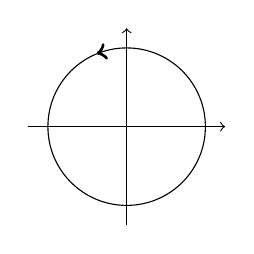
\begin{tikzpicture}[scale=0.5]

\draw[->] (0,-2.5) --(0,2.5);
\draw[->] (-2.5,0) --(2.5,0);
\draw[->, very thick] (-0.74,1.8625) --(-0.75,1.86);
\draw[] (0,0) circle (2);
\end{tikzpicture}
\end{center}
\columnbreak
\null\vfill
\begin{align*}
C(t)&=\left( \cos(t),\sin(t)\right)\\
t&\in(0,2\pi]
\end{align*}
\null\vfill
\end{multicols}



\begin{align*}
\int\limits_C vds  = & \int\limits_0^{2\pi } { < v\left( {C\left( t \right)} \right),C^1\left( t \right) > dt} \\
= & \int\limits_0^{2\pi } \left( -\sin t,\cos t\right)\cdot  \left( {\begin{array}{*{20}{c}}
{ - \sin t}\\
{\cos t}
\end{array}} \right) dt\\
= & \int\limits_0^{2\pi } \left( \sin^2 t+\cos^2 t\right) dt=2\pi\not= 0\\
\Rightarrow &\text{ $v$ auf $\Omega$ ist nicht konservativ!}
\end{align*}
Jetzt betrachten wir $\Omega'=\left\{ \left( x,y\right) \mid x>0 \right\}$ \todo{can't understand image on page 187, top} und führen Polarkoordinaten ein \[x=r\cos\theta, y=r\sin\theta\hspace{10mm} -\frac{\pi}{2}<\theta <\frac{\pi}{2}\]
Dann ist $\tan\theta = \frac{y}{x}$ und \[\theta=\arctan\frac{y}{x}\]
Wir betrachten $\theta:\Omega'\to\R$ als ein Funktion der Variablen $x,y$ und berechnen
\begin{align*}
\frac{{\partial \theta }}{{\partial x}} = & \frac{1}{{1 + {{\left( {\frac{y}{x}} \right)}^2}}}\left( { - \frac{y}{{{x^2}}}} \right) =  - \frac{y}{{{x^2} + {y^2}}}\\
\frac{{\partial \theta }}{{\partial x}} = & \frac{x}{{{x^2} + {y^2}}}
\end{align*}
Also gilt
\[\nabla \theta\left( x,y\right) = v\left( x,y\right)\]
\[v\left( x,y\right) \in\Omega'\]
$$\Rightarrow\text{ $v$ ist konservative auf $\Omega$}$$
Das heisst die Konservativität ist eine Eigenschaft zugleich des Vektorfeldes $v$ \underline{v} und der Region $\Omega$.
\end{enumerate}

\begin{definition}{8.49}
Eine offene Menge $\Omega\subset\R^n$ heisst einfach zusammenhängend, falls
\begin{enumerate}
\item $\Omega$ ist stückweise $C^1-$wegzusammenhängend
\item Jeder stückweise $C^1-$Weg in $\Omega$ kann stetig innerhalb $\Omega$ auf einen Punkt zusammengezogen werden
\end{enumerate}
Die Region $\Omega=\R\backslash\{ 0\}$ ist nicht einfach zu $\Omega' = \left\{ \left( x,y\right) \mid x>0\right\}$ ist es aber.\todo[inline]{limenet: This sentence doesn't make any sense at all}%DO NOT MODIFY THIS TODO AS IT MESSES UP FLOATS WHEN BUILDING
\end{definition}

\subsubsection*{Satz 8.50}
Sei $\Omega\in\R^2$ beschränkt zusammenhängend sowie einfachzusammenhängend, sei $v\in C^1\left( \Omega:\R^2\right)$ Vektorfeld. Dann sind folgende Aussagen äquivalent
\begin{enumerate}
\item $v$ ist konservativ
\item $\frac{\partial v_1}{\partial y}=\frac{\partial v_2}{\partial x}$
\end{enumerate}

\subsection*{Taylorentwicklung und das lokale Verhalten von $C^m-$Funktionen}\todo[inline]{Not sure how big of a title...}
Wir werden jetzt ein Verallgemeinerung der Taylorentwicklung einer Variablen herleiten. \\

Sei $f:\R^n\to\R$ eine $C^m-$Funktion sowie $x_0,x_1\in\R^n$. (Allgemein könnte man $\R^n$ durch eine offene konvexe Menge ersetzen)\\

\noindent Sei
\begin{align*}
\varphi:\R &\to\R^n\\
t & \to \left( 1-t\right) x_0+x_1
\end{align*}
Dann ist $g:=f\circ\varphi:\R\to\R$ eine \todo[inline]{Don't know where this actually fits: $\left( g(0)=f=\left( x_0\right), g(1)=f\left( x_1\right)\right)$}$C^m-$Funktion und (nach Taylorentwicklung \todo{can't read, page 189 bottom} von Funktionen mit einer Variablen) gibt es $\xi\in (0,1)$, so dass

\[
g\left( {} \right) = g\left( 0 \right) + g'\left( 0 \right) +  \ldots  + \frac{{{g^{\left( {m - 1} \right)}}\left( 0 \right)}}{{\left( {m - 1} \right)!}} + \frac{{{g^{\left( m \right)}}\left( \xi  \right)}}{{m!}}\tag{\textasteriskcentered\label{Chap8Equation,Taylor}}
\]
\todo[inline]{can't read between brackets before equal sign, page 190 very top}
Jetzt berechnen wir $g^{(i)}(t)$ als Funktion von $f$ und deren Ableitungen. Für $g'(t)$ benutzen wir die Kettenregel:
\[g'(t)=df\left( \varphi (t)\right) \cdot\varphi' (t)\] mit \[\varphi '(t) = {x_1} - {x_0} = \left( {{x_1}' - {x_0}',{x_1}^2 - {x_0}^2, \ldots ,{x_1}^n - {x_0}^n} \right)\] Erhalten wir:

\begin{align*}
g'(t) = & \sum\limits_{i = 1}^n {\frac{{\partial f}}{{\partial {x^i}}}\left( {\varphi (t)} \right)\left( {x_1^i - x_0^i} \right)}  = \nabla f\left( {\varphi (t)} \right) \cdot \left( {{x_1} - {x_0}} \right)\\
g'(0) = & \sum\limits_{i = 1}^n {\frac{{\partial f}}{{\partial {x^i}}}\left( {x_0} \right)\left( {x_1^i - x_0^i} \right)}  = \nabla f\left( {x_0} \right) \cdot \left( {{x_1} - {x_0}} \right)
\end{align*}
Jetzt berechnen wir $g^{(2)}(t)$:\[{g^{(2)}}(t) = \frac{d}{{dt}}\left( {g'\left( t \right)} \right) = \sum\limits_{i = 1}^n {\frac{d}{{dt}}\left( {\frac{{\partial f}}{{\partial {x^i}}}\left( {\varphi \left( t \right)} \right)} \right)} \left( {x_1^i - x_0^i} \right)\]
Analog gilt:
\[\frac{d}{{dt}}\left( {\frac{{\partial f}}{{\partial {x^i}}}\left( {\varphi \left( t \right)} \right)} \right) = \sum\limits_{j = 1}^n {\frac{{{\partial ^2}f}}{{\partial {x^j}\partial {{\text{x}}^i}}}\left( {\varphi \left( t \right)} \right)\left( {x_1^j - x_0^j} \right)} \]
Eingesetzt gilt:
\begin{align*}
{g^{(2)}}(t) = & \sum\limits_{i = 1}^n {\sum\limits_{j = 1}^n {\left( {\frac{{{\partial ^2}f}}{{\partial {x^j}\partial {x^i}}}\left( {\varphi (t)} \right)} \right)} } \left( {x_1^i - x_0^i} \right)\left( {x_1^j - x_0^j} \right)\\
{g^{(2)}}(0) = & \sum\limits_{i,j = 1}^n {\left( {\frac{{{\partial ^2}f}}{{\partial {x^j}\partial {x^i}}}\left( {{x_0}} \right)} \right)} \left( {x_1^i - x_0^i} \right)\left( {x_1^j - x_0^j} \right)
\end{align*}
Daraus schliesst man induktiv, dass
\[{g^{(k)}}(t) = \sum\limits_{{i_1},{i_2}, \ldots ,{i_k} = 1}^n {\left( {\frac{{{\partial ^k}f}}{{\partial {x^{{i_1}}} \ldots \partial {x^{{i_k}}}}}\left( {\varphi (t)} \right)} \right)} \prod\limits_{l = 1}^k {\left( {x_1^{{i_l}} - x_0^{{i_l}}} \right)} \]
Eingesetzt in (\textasteriskcentered) (s.\pageref{Chap8Equation,Taylor}) ergibt \todo[inline]{MISSING CONTENT?? page 191 bottom}

\subsubsection*{Satz 8.51(Taylorentwicklung)}
\begin{align*}
f\left( {{x_1}} \right) = & f\left( {{x_0}} \right) + \sum\limits_{i = 1}^n {\frac{{\partial f}}{{\partial x'}}\left( {{x_0}} \right)\left( {x_1^i - x_0^i} \right) +  \ldots } \\
 + & \frac{1}{{\left( {m - 1} \right)!}}\sum\limits_{{i_1}, \ldots ,{i_{m - 1}} = 1}^n {\frac{{{\partial ^{m - 1}}f}}{{\partial {x^{{i_1}}} \ldots \partial {x^{{i_{m - 1}}}}}}\left( {{x_0}} \right)\prod\limits_{l = 1}^{\left( {m - 1} \right)} {\left( {x_1^{{i_l}} - x_0^{{i_l}}} \right)} } \\
 + & \frac{1}{{m!}}\sum\limits_{{i_1}, \ldots ,{i_m} = 1}^n {\frac{{{\partial ^m}f}}{{\partial {x^{{i_1}}} \ldots \partial {x^{{i_m}}}}}\left( {{x_\xi }} \right)\prod\limits_{l = 1}^m {\left( {x_1^{{i_l}} - x_0^{{i_l}}} \right)} }
\end{align*}
mit einer Zahl $\xi\in\left( 0,1\right)$, $x_\xi = \left( 1-\xi\right)x_0+\xi x_1$.

\subsubsection*{Bemerkung 8.52}
Insbesondere für $m=2$ erhalten wir für $f$ die quadratische Näherung
\begin{align*}
f\left( {{x_1}} \right) = & f\left( {{x_0}} \right) + \nabla f\left( {{x_0}} \right)\left( {{x_1} - {x_0}} \right)\\
 + &\frac{1}{2}\sum\limits_{i,j = 1}^2 {\frac{{{\partial ^2}f}}{{\partial {x^i}\partial {x^j}}}\left( {{x_0}} \right)\left( {x_1^i - x_0^i} \right)} \left( {x_1^j - x_0^j} \right) + {r_2}\left( {f,{x_1},{x_0}} \right)
\end{align*}
mit Fehler
\[\frac{r_2\left( f,y_1,x_0\right)}{\abs{ x_1-x_0}}\to 0, \left( x_1\to x_0\right)\]

\begin{definition}{8.53}
Die Matrix der zweiten partiellen Ableitungen heisst Hesse - Matrix von $f$ und wird mit $\Hess(f)$ oder $\nabla^2 f$ bezeichnet
\begin{align*}
\Hess(f)= & \nabla^2 f:=\left( \frac{\partial^2 f}{\partial x^i\cdot\partial x^j}\right)_{i,j=1\dots n}\\
 = & \left( {\begin{array}{*{20}{c}}
{\frac{{{\partial ^2}f}}{{\partial x'\partial x'}}}&{\frac{{{\partial ^2}f}}{{\partial x'\partial {x^2}}}}& \ldots &{\frac{{{\partial ^2}f}}{{\partial x'\partial {x^n}}}}\\
{\frac{{{\partial ^2}f}}{{\partial {x^2}\partial x'}}}&{\frac{{{\partial ^2}f}}{{\partial {x^2}\partial {x^2}}}}& \ldots &{\frac{{{\partial ^2}f}}{{\partial {x^2}\partial {x^n}}}}\\
 \vdots & \vdots & \ddots & \vdots \\
{\frac{{{\partial ^2}f}}{{\partial {x^n}\partial x'}}}& \ldots & \ldots &{\frac{{{\partial ^2}f}}{{\partial {x^n}\partial {x^n}}}}
\end{array}} \right)
\end{align*}
\end{definition}
Seien $\nabla f,x_1-x_0$ Zeilenvektoren und sei $\left( x-x_0\right)^t$ der zu $x_1-x_0$ transponierte Spaltenvektor . Dann wird die Taylorentwicklung von Grad 2 äquivalent zu

\begin{align*}
f(x) = & f\left( x_0\right) + \nabla f\left( x_0\right) \left( x-x_0\right)^t\\
+ & \frac{1}{2}\left( x-x_0\right)\cdot\nabla^2 f\left( x_0\right)\left( x-x_0\right)^t\\
+ & r_3\left( f,x,x_0\right)
\end{align*}

\subsubsection*{Bemerkung}
Die Hesse - Matrix von $f$ ist nach Satz von Schwarz eine symmetrische Matrix.

\subsubsection*{Beispiel}
$f\left( x,y\right)=e^{x+y}\cos x$ im Punkt $(0,0)$. Die Taylorentwicklung vom Grad 2:
\begin{align*}
\frac{{\partial f}}{{\partial x}} = & {e^{x + y}}\cos x - {e^{x + y}}\sin x,\text{ }\frac{{\partial f}}{{\partial x}}(0,0) = 1\\
\frac{{\partial f}}{{\partial x}} =  & {e^{x + y}}\cos x ,\text{ }\frac{{\partial f}}{{\partial x}}(0,0) = 1\\
\end{align*}
\todo[inline]{shouldn't it be $\frac{{\partial f}}{{\partial y}}(0,0) = 1$ for second one??}
\[\left( \nabla f\right)(0,0)=(1,1)\hspace{10mm}f(0,0)=1\]
\begin{align*}
\frac{\partial }{{\partial x}}\left( {\frac{{\partial f}}{{\partial y}}} \right) = & {e^{x + y}}\cos x - {e^{x + y}}\sin x,\text{ }\frac{{{\partial ^2}f}}{{\partial x\partial y}}(0,0) = 1\\
\frac{{\partial^2 f}}{{\partial x^2}} = \frac{\partial }{{\partial x}}\left( {\frac{{\partial f}}{{\partial x}}} \right) = & {e^{x + y}}\cos x - {e^{x + y}}\sin x - {e^{x + y}}\sin x - {e^{x + y}}\cos x\\
= & -2e^{x+y}\sin x\\
\frac{{{\partial ^2}f}}{{\partial {x^2}}}(0,0) = & 0\\
\frac{{{\partial ^2}f}}{{\partial {y^2}}} = & {e^{x + y}}\cos x\hspace{10mm}\frac{{{\partial ^2}f}}{{\partial {y^2}}}(0,0) = 1
\end{align*}
\[{\nabla ^2}f(0,0) = \left( {\begin{array}{*{20}{c}}
0&1\\
1&1
\end{array}} \right)\]

\begin{align*}
\left( {\left( {x,y} \right) - \left( {0,0} \right)} \right){\nabla ^2}f\left( {0,0} \right){\left( {\left( {x,y} \right) - \left( {0,0} \right)} \right)^T} = & \left( {x,y} \right)\left( {\begin{array}{*{20}{c}}
0&1\\
1&1
\end{array}} \right)\left( {\begin{array}{*{20}{c}}
x\\
y
\end{array}} \right)\\
 = & \left( {x,y} \right)\left( {\begin{array}{*{20}{c}}
y\\
{x + y}
\end{array}} \right)\\
 = &\text{ }2xy+y^2
\end{align*}
\begin{align*}
f\left( {x,y} \right) = & \text{ }{e^{x + y}}\cos x = 1 + \left( {\begin{array}{*{20}{c}}
1\\
1
\end{array}} \right)\left( {x,y} \right) + \frac{1}{2}\left( {x,y} \right)\left( {\begin{array}{*{20}{c}}
0&1\\
1&1
\end{array}} \right)\left( {\begin{array}{*{20}{c}}
x\\
y
\end{array}} \right)\\
 = & \text{ } 1 + \left( {x,y} \right) + \frac{1}{2}\left( {2xy + {y^2}} \right) + {r_3}\left( {f,\left( {x,y} \right)} \right)
\end{align*}
Taylorpolynom von Grad 2: $1+\left( x+y\right)+\frac{1}{2}\left( 2xy+y^2\right)$\\

Die Hesse - Matrix bestimmt, ob die Funktion $f$ in der Nähe von $x$ konvex oder konkav ist (oder nicht). Sie spielt die gleiche Rolle wie die zweite Ableitung von Funktionen in einer Variable. \\

Als nächstes benötigen wir eine mehrdimensionale Entsprechung zur Positivität \todo{Can't understand word between brackets, page 197 middle} in den eindimensionalen Beziehungen $f''(z)>0$ bzw. $f''(z)<0$.

\begin{definition}{8.54}
Eine symmetrische Matrix $A=\left( a_{ij}\right)\in\R^{n\times n}$ heisst
\begin{enumerate}
\item \textbf{Positiv definit} wenn \[{}^txAx = \sum\limits_{i,j = 1}^n {{a_{ij}}{x^i}{x^j} > 0}\hspace{10mm}\forall x\in\R^n\] (oder wenn sämtliche Eigenwerte positive sind)
\item \textbf{Negativ definit} wenn \[{}^txAx < 0\hspace{10mm}\forall x\in\R^n\] (wenn sämtliche Eigenwerte negativ sind)
\item Sonst \textbf{indefinit} (wenn sie sowohl positive als auch negative Eigenwerte besitzt)
\end{enumerate}
Im symmetrischen $2\times 2$ Fall ist die Gleichung auf Definitheit besonders leicht
\end{definition}

\subsubsection*{Satz 8.55}
Eine Symmetrische Matrix
\[A = \left( {\begin{array}{*{20}{c}}
{{a_{11}}}&{{a_{12}}}\\
{{a_{12}}}&{{a_{11}}}
\end{array}} \right)\]
ist genau dann
\begin{enumerate}
\item Positiv definit, wenn $\det A>0$ und $a_{11}>0$
\item Negativ definit, wenn $\det A>0$ und $a_{11}<0$
\item Indefinit, wenn $\det A<0$
\end{enumerate}

\subsection*{Extrema von Funktionen mehrerer Variablen}
Jetzt werden wir nach Punkten $x\in\R^n$ schauen, in denen eine Funktion $F:\R^n\to\R$ ein lokales Extremum annimmt. Wir erinnern uns an das Vorgehen im $f:\R\to\R$:
\begin{enumerate}
\item Finde alle Punkte $x\in\R$, für die $f'(x)=0$ gilt (Notwendige Bedingung)
\item Falls in einem solchen Punkt zusätzlich $f''(x)>0$ (bzw. $f''(z)<0$) gilt, so handelt es sich um ein lokales Minimum (bzw. Maximum) (hinreichende Bedingung)
\end{enumerate}
Jetzt verallgemeinern wir diese Strategie. Zunächst:

\begin{definition}{8.55}
Ein Punkt $x_0\in\R^n$ mit $df\left( x_0\right)=0$ heisst \underline{kritischer Punkt} von $f$ (oder \underline{stationärer} Punkt von $f$)
\end{definition}

\subsubsection*{Satz 8.56}
Sei
\begin{align*}
f: &\text{ } \Omega \subset\R^n\to\R\\
f \in & \text{ }C^2\left(\Omega\right); x_0\in\Omega
\end{align*}
\begin{enumerate}
\item Falls $x_0\in\Omega$ ein lokale Extremum (Minimum oder Maximum) von $f$ ist, so gilt $df\left(x_0\right)=0$
\item Falls $df\left( x_0\right)=0$, und falls $\Hess \left( f\right)\left( x_0\right)$ positiv definit ist, so ist $x_0$ eine lokale Minimalstelle
\item Falls $df\left( x_0\right)$, und falls $\Hess_f\left( x_0\right)<0$ negativ definit ist, so ist $x_0$ eine lokale Maximalstelle
\item Falls $df\left( x_0\right)=0$, und $\Hess_f\left( x_0\right)$ indefinit ist, so ist $x_0$ ein Sattelpunkt (d.h. jede Umgebung $U$ von $x_0$ enthält Punkte $p,q\in U$ mit $f\left( P\right) > f\left( x_0\right)>f\left( q\right)$)
\end{enumerate}

\subsubsection*{Beispiel}
\begin{enumerate}
\item \begin{align*}
f\left( x,y,z\right)= & \left(x-1\right)^2+\left(y+2\right)^2+\left(z+1\right)^2\\
\nabla f= & \left( 2\left(x-1\right),2\left(y+2\right),2\left(z+1\right)\right)\\
\nabla f\left( x_0\right)&=\left( 0,0,0\right)\Rightarrow x_0=\left( 1,-2,-1\right)
\end{align*}
\[{H_f}\left( {{x_0}} \right) = \left( {\begin{array}{*{20}{c}}
2&0&0\\
0&2&0\\
0&0&2
\end{array}} \right)\]
$H_f\left( x_0\right)$ ist positiv definit $\Rightarrow x_0\left( 1,-2,-1\right)$ ist ein lokales Minimum.
\item \begin{align*}
f\left( x,y\right)= & \cos\left(x+2y\right)+\cos\left(2x+3y\right)\\
\nabla f= & \left( -\sin\left(x+2y\right)-2\sin\left( 2x +3y\right)\right.,\\
&\left.-2\sin\left(x+2y\right)-3\sin\left(2x+3y\right)\right)=\left( 0,0\right)\\
\Rightarrow &-\sin\left( x+2y\right)-2\sin\left( 2x+3y\right)=0\\
&-2\sin\left( x+2y\right)-3\sin\left( 2x+3y\right)=0
\end{align*}
\[\Rightarrow \sin\left( 2x+3y\right) = 0,\text{ }\sin\left( x+2y\right)=0\]
\[ \Rightarrow \left. {\begin{array}{*{20}{r}}
{2x + 3y = k\pi }\\
{x + 2y = l\pi }
\end{array}} \right\} \Rightarrow y = k\pi {\text{ und }}x = l\pi \]
Kritische Punkte: $\left( \pi l,\pi k\right)\hspace{5mm}k,l\in\mathbb{Z}$
\begin{align*}
\frac{{\partial f}}{{\partial y\partial x}} &=\frac{{\partial f}}{{\partial x\partial y}} =  - 2\cos \left( {x + 2y} \right) - 6\cos \left( {2x + 3y} \right)\\
\frac{{{\partial ^2}f}}{{\partial {x^2}}} &=- \cos \left( {x + 2y} \right) - 4\cos \left( {2x + 3y} \right)\\
\frac{{{\partial ^2}f}}{{\partial {y^2}}} &=- 4\cos \left( {x + 2y} \right) - 9\cos \left( {2x + 3y} \right)
\end{align*}
\[\left( 0,0\right):\frac{{{\partial ^2}f}}{{\partial {x^2}}}=-5<0\]
\[\abs{ {{\nabla ^2}f\left( {0,0} \right)} } = \left| {\begin{array}{*{20}{c}}
{ - 5}&{ - 8}\\
{ - 8}&{ - 13}
\end{array}} \right| = 13 \cdot 5 - 64 = 1 < 0\]
$\Rightarrow\nabla^2 f\left( 0,0\right)$ ist negativ definit und $\left( 0,0\right)$ ist eine lokale Maximalstelle.\\

Auch alle Punkte $\left( -2\pi k,2\pi l\right)$ sind lokale Maxima. Analog, bis auf Addition von Vielfachen von $2\pi$, hat $f$ eine lokale Minimalestelle in $\left( \pi,\pi\right)$ und Sattelpunkte in $\left( 0,\pi\right)$ und $\left( \pi,0\right)$
\end{enumerate}

\section{Vektorwertige Funktionen}
Sei $\Omega\in\R^n$, $f=\left( f^i\right)_{1 < i < l}\Omega\to\R^l$
\begin{definition}{8.57}
\begin{enumerate}
\item Die Funktion \todo[inline]{can,t understand the function, page 203 top} heisst an der Stelle $x_0\in\Omega$ differenzierbar, falls jede Komponente $f^i$, $1 < i < l$ an der stelle $x_0$ differenzierbar ist.\\

Das Differential $df\left( x_0\right)$ hat die Gestalt \[df\left( {{x_0}} \right) = \left( {\begin{array}{*{20}{c}}
{df'\left( {{x_0}} \right)}\\
{d{f^n}\left( {{x_0}} \right)}
\end{array}} \right)\]
\item $f$ heisst auf $\Omega$ differenzierbar (bzw. von der Klasse $C^m$, $m\geq 1$) falls jedes $f^i$ differenzierbar ist (bzw. $f^i\in C^m\left( \Omega\right)$) $1\leq i \leq l$
\end{enumerate}
\end{definition}
\subsubsection*{Bemerkung 8.58}
\begin{enumerate}
\item Bezüglich der Standardbasis $dx^j$, $1\leq j\leq n$ erhalten wir
\[d{f^i}\left( {{x_0}} \right) = \sum\limits_{j = 1}^n {\frac{{\partial {f^i}}}{{\partial {x^j}}}\left( {{x_0}} \right)d{x^j} = \left( {\frac{{\partial {f^i}}}{{\partial x'}}\left( {{x_0}} \right), \ldots ,\frac{{\partial {f^i}}}{{\partial {x^n}}}\left( {{x_0}} \right)} \right)} \]
die Darstellung
\[df\left( {{x_0}} \right) = \left( {\begin{array}{*{20}{c}}
{\frac{{\partial f'}}{{\partial x'}}\left( {{x_0}} \right)}&{\frac{{\partial f'}}{{\partial {x^2}}}\left( {{x_0}} \right)}& \ldots &{\frac{{\partial f'}}{{\partial {x^n}}}\left( {{x_0}} \right)}\\
{\frac{{\partial {f^2}}}{{\partial x'}}\left( {{x_0}} \right)}&{\frac{{\partial {f^2}}}{{\partial {x^2}}}\left( {{x_0}} \right)}& \ldots &{\frac{{\partial {f^2}}}{{\partial {x^n}}}\left( {{x_0}} \right)}\\
 \vdots & \vdots & \ddots & \vdots \\
{\frac{{\partial {f^l}}}{{\partial x'}}\left( {{x_0}} \right)}&{\frac{{\partial {f^l}}}{{\partial x'}}\left( {{x_0}} \right)}& \ldots &{\frac{{\partial {f^l}}}{{\partial {x^n}}}\left( {{x_0}} \right)}
\end{array}} \right)\]
Die $l\times n$ matrix $df\left( x_0\right) = {\left( \frac{\partial f^i}{\partial x^j}\left( x_0\right)\right)}_{1\leq i\leq l, 1\leq j\leq n}$ heisst Jacobi- oder Funktionalmatrix von $f$ an der Stelle $x_0$.
\item Auch im vektorwertigen Fall ist die Funktion $f$ genau dann differenzierbar in $x_0$, wenn eine lineare Abbildung $A:\R^n\to\R^l$ existiert mit
\[\mathop {\lim }\limits_{x \to {x_0}} \frac{{f\left( x \right) - f\left( {{x_0}} \right) - A\left( {x - {x_0}} \right)}}{{\abs{ {x - {x_0}} }}} = 0\]
\end{enumerate}

\subsubsection*{Beispiel 8.59}

\begin{enumerate}
\item \[f:\R^2\to\R\]
\[f\left( {x,y} \right) = \left( {\begin{array}{*{20}{c}}
{{x^2} - {y^2}}\\
{2xy}
\end{array}} \right)\]
\[f\in C^\infty\left( \R^2:\R^2\right) \text{ mit } df\left( {x,y} \right) = \left( {\begin{array}{*{20}{c}}
{2x}&{ - 2y}\\
{2y}&{2x}
\end{array}} \right) \]
\item Polarkoordinaten
\begin{align*}
f&:\lbrack 0,\infty)\times\lbrack 0,2\pi\rbrack\to\R^2\\
\left( {\begin{array}{*{20}{c}}
r\\
\theta
\end{array}} \right) &\to \left( {\begin{array}{*{20}{c}}
x\\
y
\end{array}} \right) = \left( {\begin{array}{*{20}{c}}
{r\cos \theta }\\
{r\sin \theta }
\end{array}} \right) = \left( {\begin{array}{*{20}{c}}
{f'}\\
{{f^2}}
\end{array}} \right)\\
df'\left( r,\theta\right)&=\left( \cos\theta, -r\sin\theta\right)\\
df^2\left( r,\theta\right)&=\left( \sin\theta, r\cos\theta\right)\\
df\left( {r,\theta } \right) &= \left( {\begin{array}{*{20}{c}}
{\cos \theta }&{ - r\sin \theta }\\
{\sin \theta }&{r\cos \theta }
\end{array}} \right) \leftarrow {\text{Jacobi Matrix}}\\
\det\left( df\left( r,\theta\right)\right)&=r\left( \cos^2\theta + \sin^2\theta\right)=r
\end{align*}

\begin{center}
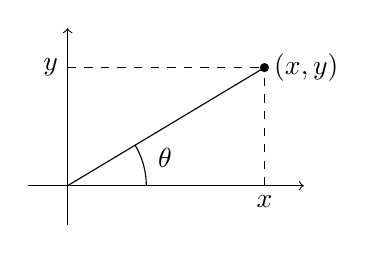
\begin{tikzpicture}

\draw[->] (0,-0.5) --(0,2);
\draw[->] (-0.5,0) --(3,0);

\draw (0,0) --(2.5,1.5);
\draw[fill=black] (2.5,1.5) circle (0.05);
\draw (1,0) arc (0:31:1cm); 

\draw[dashed] (0,1.5) --(2.5,1.5);
\draw[dashed] (2.5,0) --(2.5,1.5);
\draw(2.5,0) node [anchor=north]{$x$};
\draw(0,1.5) node [anchor=east]{$y$};
\draw(2.5,1.5) node [anchor=west]{$(x,y)$};
\draw(1.45,0.35) node [anchor=east]{$\theta$};
\end{tikzpicture}
\end{center}

\begin{center}
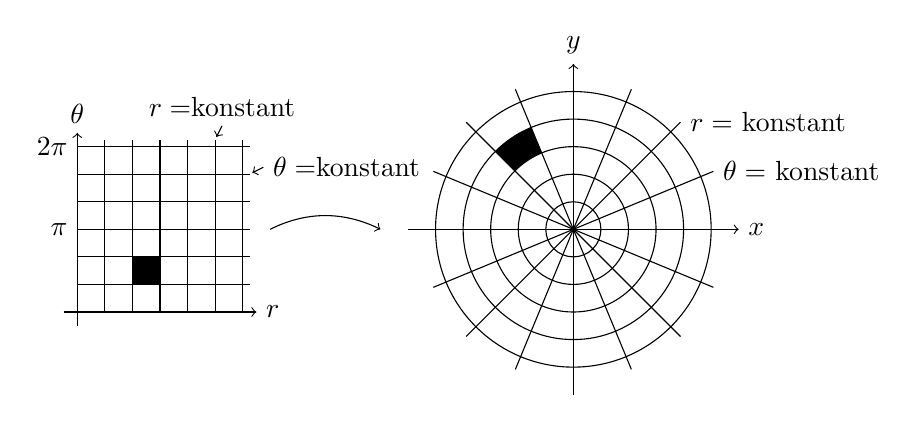
\begin{tikzpicture}[scale=0.35]

\fill[fill=black]
    (18,3) -- ++(4cm,0cm) arc (0:135:4cm);

\fill[fill=white]
    (18,3) -- ++(3cm,0cm) arc (0:135:3cm);

\fill[fill=white]
    (18,3) -- ++(4cm,0cm) arc (0:112.5:4cm);

\draw[->] (0,-0.5) --(0,6.5);
\draw[->] (-0.5,0) --(6.5,0);

\draw (1,0) --(1,6.25);
\draw (2,0) --(2,6.25);
\draw (3,0) --(3,6.25);
\draw (4,0) --(4,6.25);
\draw (5,0) --(5,6.25);
\draw (6,0) --(6,6.25);

\draw (0,1) --(6.25,1);
\draw (0,2) --(6.25,2);
\draw (0,3) --(6.25,3);
\draw (0,4) --(6.25,4);
\draw (0,5) --(6.25,5);
\draw (0,6) --(6.25,6);

\draw (0,6.5) node [anchor=south]{$\theta$};
\draw (6.5,0) node [anchor=west]{$r$};
\draw (0,3) node [anchor=east]{$\pi$};
\draw (0,6) node [anchor=east]{$2\pi$};

\draw [fill=black] (2,1)--(2,2)--(3,2)--(3,1);

\draw [<-] (6.35,5.05) --(6.75,5.25);
\draw (6.75,5.25) node [anchor =west]{$\theta=$konstant};

\draw [<-] (5.05,6.35) --(5.25,6.75);
\draw (5.25,6.75) node [anchor =south]{$r=$konstant};

\draw[->](7,3)parabola bend (9,3.5)(11,3);


\draw[->] (18,-3) --(18,9);
\draw[->] (12,3) --(24,3);
\draw[] (18,3) circle (1);
\draw[] (18,3) circle (2);
\draw[] (18,3) circle (3);
\draw[] (18,3) circle (4);
\draw[] (18,3) circle (5);

\draw (18,3) -- ++(45:5.5) node [anchor=west] {$r=$ konstant};
\draw (18,3) -- ++(135:5.5);
\draw (18,3) -- ++(225:5.5);
\draw (18,3) -- ++(315:5.5);

\draw (18,3) -- ++(45+22.5:5.5);
\draw (18,3) -- ++(135+22.5:5.5);
\draw (18,3) -- ++(225+22.5:5.5);
\draw (18,3) -- ++(315+22.5:5.5);

\draw (18,3) -- ++(45-22.5:5.5) node [anchor=west] {$\theta=$ konstant};
\draw (18,3) -- ++(135-22.5:5.5);
\draw (18,3) -- ++(225-22.5:5.5);
\draw (18,3) -- ++(315-22.5:5.5);

\draw (24,3) node [anchor=west] {$x$};
\draw (18,9) node [anchor=south] {$y$};

\end{tikzpicture}
\end{center}
\item Zylinderkoordinaten

\begin{multicols}{2}
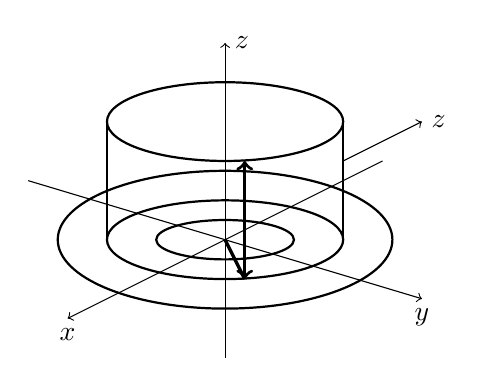
\begin{tikzpicture}[scale=0.5]

\draw[->] (0,-3) --(0,5);
\draw[->] (-5,1.5) --(5,-1.5);
\draw[->] (4,2) -- (-4,-2);


\draw[thick] (0,0) ellipse (3 and 1);
\draw[thick] (0,3) ellipse (3 and 1);
\draw[thick] (3,0) --(3,3);
\draw[thick] (-3,0) --(-3,3);
\draw[thick] (0,0) ellipse (4.25 and 1.75);
\draw[thick] (0,0) ellipse (1.75 and 0.5);

\draw (0,5) node[anchor=west]{$z$};
\draw (5,-1.5) node[anchor=north]{$y$};
\draw (-4,-2) node[anchor=north]{$x$};

\draw[->] (3,2) -- (5,3);
\draw (5,3) node[anchor=west]{$z$};

\draw[very thick](0,0) -- (0.5,-1);
\draw[very thick,<->](0.5,-1) --(0.5,2);
\end{tikzpicture}
\columnbreak
\null\vfill
Die $x,y$ Anteile werde in Polarkoordinaten transformiert und die $z$-Koordinate beibehalten
\null\vfill
\end{multicols}
\begin{align*}
f:&\lbrack 0,\infty\rbrack\to\lbrack 0,2\pi\rbrack\times\R\to\R^2\\
\left( {\begin{array}{*{20}{c}}
r\\
\theta \\
z
\end{array}} \right) \to& \left( {\begin{array}{*{20}{c}}
x\\
y\\
z
\end{array}} \right) = \left( {\begin{array}{*{20}{c}}
{r\cos \theta }\\
{r\sin \theta }\\
z
\end{array}} \right) = \left( {\begin{array}{*{20}{c}}
{f'}\\
{{f^2}}\\
{{f^3}}
\end{array}} \right)\\
df(r,\theta ,z) &=\left[ {\begin{array}{*{20}{c}}
{\cos \theta }&{ - r\sin \theta }&0\\
{\sin \theta }&{r\cos \theta }&0\\
0&0&1
\end{array}} \right] \leftarrow {\text{Jacobi Matrix}}\\
\det \left( {df(r,\theta ,z)} \right) &=r\left( {{{\cos }^2}\theta  + si{n^2}\theta } \right) = r
\end{align*}
\centerline{(Rotationssymmetrie bezüglich $z$ Achse)}
\item Kugelkoordinaten

\begin{center}
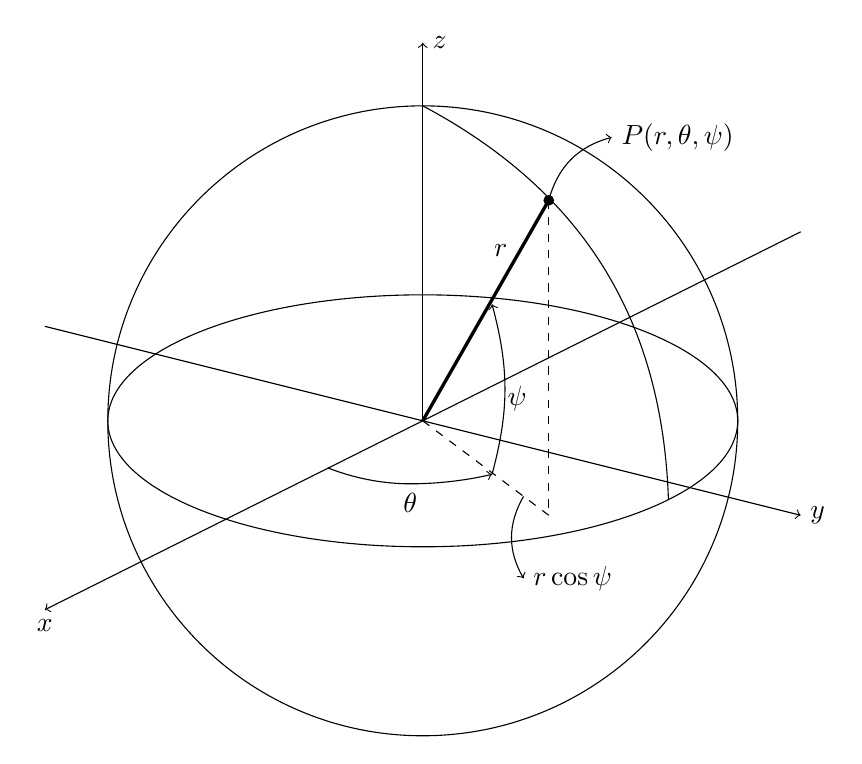
\begin{tikzpicture}[scale=0.8]

\draw[->] (0,0) --(0,6) node [anchor=west]{$z$};
\draw[->] (-6,1.5) --(6,-1.5) node [anchor=west]{$y$};
\draw[->] (6,3) -- (-6,-3) node [anchor=north]{$x$};

\draw[] (0,0) ellipse (5 and 2);
\draw[] (0,0) circle (5);

\draw[very thick](0,0)--(2,3.5);
\draw[fill=black] (2,3.5) circle (0.075);
\draw[bend left,->](2,3.5) to (3,4.5) node [anchor=west]{$P(r,\theta,\psi)$};
\draw[dashed](2,3.5)--(2,-1.5);
\draw[dashed](0,0)--(2,-1.5);
\draw[->](-1.5,-0.75) parabola bend (-0.2,-1)(1.1,-0.85);
\draw (-0.2,-1) node [anchor=north]{$\theta$};
\draw [->, bend right=15] (1.1,-0.85) to (1.1,1.85);
\draw (1.5,0.7) node [anchor=north]{$\psi$};
\draw[bend right,->](1.6,-1.2) to (1.6,-2.5) node[anchor=west]{$r\cos\psi$};
\draw (1.5,2.7) node [anchor=east]{$r$};
\draw[bend left](0,5) to (3.9,-1.25);
\end{tikzpicture}

\end{center}


\begin{align*}
f:&\lbrack 0,\infty)\times\lbrack 0,2\pi\rbrack\times\left(-\frac{\pi}{2},\frac{\pi}{2}\right)\to\R^3\\
f\left( {\begin{array}{*{20}{c}}
r\\
\theta \\
\psi
\end{array}} \right) &=\left( {\begin{array}{*{20}{c}}
{r\cos \theta \cos \psi }\\
{r\sin \theta \cos \psi }\\
{r\sin \psi }
\end{array}} \right) = r\left( {\begin{array}{*{20}{c}}
{\cos \theta \cos \psi }\\
{\sin \theta \cos \psi }\\
{\sin \psi }
\end{array}} \right)\\
df\left( {r,\theta ,\psi } \right) &=\left( {\begin{array}{*{20}{c}}
{\cos \theta \cos \psi }&{ - r\sin \theta \cos \psi }&{ - r\cos \theta \sin \psi }\\
{\sin \theta \cos \psi }&{r\cos \theta \cos \psi }&{ - r\sin \theta {\mathop{\rm sin?}\nolimits} }\\
{\sin \psi }&0&{r\cos \psi }
\end{array}} \right)\\
\det\left( df\right)&=r^2cos\psi
\end{align*}
\todo{Check question mark, chopped content, page 205.3}

\begin{center}
\begin{tikzpicture}[scale=0.5]

\draw[->] (0,0) --(0,5);
\draw[->] (0,0) --(7,0);
\draw[->] (0,0) -- (-3,-3);
\draw (0,0) --(4,3);
\draw[dashed] (4,3) --(4,-2);
\draw[dashed] (0,0) --(4,-2);
\draw[fill=black] (4,3) circle (0.075);
\draw[] (4,3) node[anchor=west]{$(x,y,z)$};

\draw[->] (-1,-1) parabola bend (0.25,-1.15)(1.5,-0.75);
\draw (0.25,-1.15) node[anchor=north]{$\theta$};

\draw[] (0,5) node [anchor=south]{$z$};
\draw[] (7,0) node [anchor=west]{$y$};
\draw[] (-3,-3) node [anchor=east]{$x$};

\draw [->, bend right] (1.5,-0.75) to (1.5,1.1);
\draw (1.6,0.5) node [anchor=west]{$\psi$};
\draw (1.7,2) node [anchor=west]{$r$};

\draw[->] (3,-1.7) parabola bend (4,-3)(4,-3);
\draw (4,-3) node [anchor=west]{$r\cos\psi$};
\draw (12,2) node [anchor=south]{$\psi:$ Breitengrad};
\draw (12,2) node [anchor=north]{$\theta:$ Längengrad};

\end{tikzpicture}
\end{center}
\begin{center}
(Punktsymmetrie zum Koordinatenursprung)
\end{center}
\end{enumerate}

\noindent Es gelten die üblichen Differentiationsregeln

\subsubsection*{Satz 8.60}
Seien $f,g:\Omega\subset\R^n\to\R^l$ an der Stelle $x_0\in\Omega$ differenzierbar und $\alpha\in\R$. dann sind die Funktionen $\alpha f$ und $f+g$ sowie das Skalarprodukt von $f$ und $g$ an der Stelle $x_0$ differenzierbar und
\begin{enumerate}
\item $d\left( \alpha f\right) \left( x_0\right)=\alpha df\left( x_0\right)$
\item $d\left( f+g\right) \left( x_0\right)=df\left( x_0\right) + dg\left( x_0\right)$
\item $d\left( f\cdot g\right)\left( x_0\right) = f\left( x_0\right)\cdot dg\left( x_0\right)+g\left( x_0\right)\cdot df\left( x_0\right)$\\
wobei $f\left( x_0\right)\cdot dg\left( x_0\right)=\sum\limits_{i = 1}^l {{f^i}\left( {{x_0}} \right)d{g^i}\left( {{x_0}} \right)}$
\end{enumerate}
\subsubsection*{Satz 8.61}
Seien $g:\Omega\to\R^l$ an der Stelle $x_0\in\Omega$ und $f:\R^l\to\R^m$ an der Stelle $g\left(x_0\right)$ differenzierbar.\\

Dann ist die Funktion $f\circ g:\Omega\to\R^m$ an der Stelle $x_0$ differenzierbar, und
\[d\left( f\circ g\right)\left( x_0\right)=df\left( g\left( x_0\right)\right)\cdot dg\left( x_0\right)\]

\subsubsection*{Beispiel}
Sei
\begin{align*}
f:\R^2 & \to\R^2\\
\left( x,y\right) & \to\left( {\begin{array}{*{20}{c}}
{{x^2} - {y^2}}\\
{2xy}
\end{array}} \right) \hspace{20mm}df = \left( {\begin{array}{*{20}{c}}
{2x}&{ - 2y}\\
{2y}&{2x}
\end{array}} \right)
\end{align*}
\begin{align*}
g:\R^3 & \to\R^3\\
\left( x,y,z\right) & \to\left( {\begin{array}{*{20}{c}}
{{x^2} +{y^2}+{z^2}}\\
{xyz}
\end{array}} \right) \hspace{15mm}dg = \left( {\begin{array}{*{20}{c}}
{2x}&{2y}&{2z}\\
{yz}&{xz}&{xy}
\end{array}} \right)
\end{align*}
\begin{align*}
\left( f\circ g\right):\R^3 & \to\R^2\\
\left(x,y,z\right)&\to \left( {\begin{array}{*{20}{c}}
{{{\left( {{x^2} + {y^2} + {z^2}} \right)}^2} - {{\left( {xyz} \right)}^2}}\\
{2\left( {{x^2} + {y^2} + {z^2}} \right)\left( {xyz} \right)}
\end{array}} \right)
\end{align*}
\begin{align*}
d\left( {f \circ g} \right)\left( {x,y,z} \right)&= df\left( {g\left( {x,y,z} \right)} \right) \cdot dg\left( {x,y,z} \right)\\
&= \left( {\begin{array}{*{20}{c}}
{2\left( {{x^2} + {y^2} + {z^2}} \right)}&{ - 2xyz}\\
{2xyz}&{2\left( {{x^2} + {y^2} + {z^2}} \right)}
\end{array}} \right)\left( {\begin{array}{*{20}{c}}
{2x}&{2y}&{2z}\\
{yz}&{xz}&{xy}
\end{array}} \right)\\
&=\left( {\begin{array}{*{20}{c}}
{4x\left( {{x^2} + {y^2} + {z^2}} \right) - 2x{y^2}{z^2}}& * & * \\
 * & * & * \\
 * & * & *
\end{array}} \right)
\end{align*}
